\documentclass[a4paper, 12pt, italian]{book}
\usepackage{mathptmx}
\usepackage[T1]{fontenc}
\usepackage[utf8]{inputenc}
\usepackage[italian]{babel}
\usepackage{graphicx}
\usepackage{float}
\usepackage{amsmath}
\usepackage{mathtools}
\usepackage{amsfonts}
\usepackage{bbm}
\usepackage{enumerate}
\usepackage[margin=2cm]{geometry}
\usepackage{amsthm}
\usepackage{mathrsfs}
\usepackage{cancel}


%%%%%%%%%%%%%%%%%%%%%%%%%%%%%%%%%%%%%
%% Definizione struttura
%%%%%%%%%%%%%%%%%%%%%%%%%%%%%%%%%%%%%
\newenvironment{theorem}{Teorema: }{}
\newenvironment{exercise}{Esercizio:}{}				  
%\newenvironment{definition}{Definizione: }{}
%\newenvironment{oss}{Osservazione: }{}		
\newenvironment{example}{Esempio:}{}		
%\newenvironment{proof}{Dim:}{}	

%%%%%%%%%%%%%%%%%%%%%%%%%%%%%%%%%%%%%
%% Preamboli Ivan
%%%%%%%%%%%%%%%%%%%%%%%%%%%%%%%%%%%%%

\newcommand{\AdC}{ascisse di convergenza }
\newcommand{\RdC}{regione di convergenza }
\newcommand{\LA}{\mathscr{L}T}
\newcommand{\intZeroInfinity}{\int_{0^-}^{+\infty}}
\newcommand{\gradino}{\delta_{-1}}
\newcommand{\derN}[2]{\frac{d^{#2}#1}{dt^{#2}}}
\newcommand{\der}[1]{\frac{d#1}{dt}}
\newcommand{\NB}{I nota bene della zia wilma}

\theoremstyle{definition}
\newtheorem*{definizione}{Def}
\theoremstyle{remark}
\newtheorem*{osservazione}{Oss}
%%%%%%%%%%%%%%%%%%%%%%%%%%%%%%%%%%%%%
%% Preamboli Andrea
%%%%%%%%%%%%%%%%%%%%%%%%%%%%%%%%%%%%%
\DeclarePairedDelimiter{\abs}{\lvert}{\rvert}
\DeclarePairedDelimiter{\Abs}{\bigg\lvert}{\bigg\rvert}

% voglio compilare sono cap1_Intro.tex
%\includeonly{./capitoli/cap3_Sistemi}
% NB \includeonly va prima di \begin{document}


%%%%%%%%%%%%%%%%%%%%%%%%%%%%%%%%%%%%%
%%Inizio documento
%%%%%%%%%%%%%%%%%%%%%%%%%%%%%%%%%%%%%


\begin{document}

\begin{titlepage}

\begin{center}
\LARGE{Università degli Studi di Verona}\\
\line(1,0){450}\\
\vspace{10em}
\Huge{\textbf{Appunti di Sistemi}}\\
\vspace{14em}
\Large{di Wilma Valentino, Ivan Piazza, Laura Maule, Andrea Dall'Alba}\\
\line(1,0){450}\\
\LARGE{2019}\\
\end{center}

\end{titlepage}

\tableofcontents

\chapter{Introduzione}
\section{ Premessa }

\textbf{Def - Sistemi dinamici:}  sono un'evoluzione temporale di un ingresso e un'uscita, vengono modellati dalle \textbf{equazioni differenziali}.\\
Vedremo sono funzioni monodimensionali (cioè dipendenti solo dal tempo) ma in realtà possiamo benissimo avere più dimensioni.\\
I modelli ci danno una stima del comportamento di una sistema, in particolare il modello delle equazioni differenziali si può svolgere: nel tempo, nel dominio della trasformata di Laplace (utile con i segnali esponenziali e sinusoidali) e nel dominio della trasformata di Fourier (è un restrizione di Laplace, è utile nei segnali sinusoidali).\\
Studieremo le proprietà dei sistemi, di queste la più importante è la stabilità.\\
\textbf{Modelliamo un sistema} come fosse una scatola nera, avrà un segnale come input e output (es. suono 1D, immagine 2D).\\
I sistemi ci servono per vari motivi: possono facilitare la trasmissione di un segnale, migliorarlo accentuando alcune informazioni o eliminandone altre (filtraggio).\\
Vogliamo vedere i sistemi come \textbf{funzioni matematiche} (pag. 69 libro "")\\

\begin{figure}
	\centering
	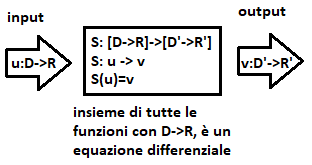
\includegraphics[width=0.7\linewidth]{sistema}
	\caption{ modello di un sistema come scatola nera}
	\label{fig:sistema}
\end{figure}



$ \forall s \in D' $ allora $ v(s)=(S(u))(s)\in R'  $ \\

\pagebreak

Abbiamo tre tipi di sistemi:\\
- Continui: operano su segnali continui\\
- Discreti: operano su segnali discreti\\
- Ibridi fra continui e discreti (non li vedremo)\\

\begin{figure}[h]
	\centering
	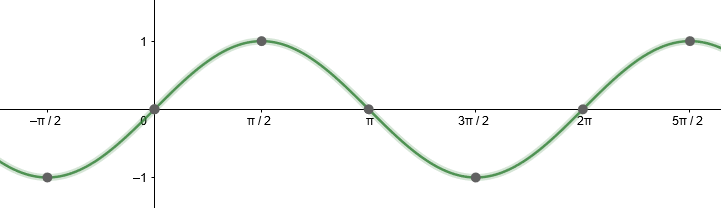
\includegraphics[width=0.7\linewidth]{seno}
	\caption{Segnale continuo}
	\label{fig:seno}
\end{figure}


\begin{figure}[h]
	\centering
	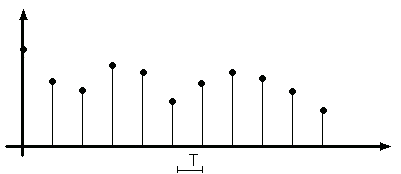
\includegraphics[width=0.7\linewidth]{tempo_discreto}
	\caption{ Segnale discreto}
	\label{fig:tempodiscreto}
\end{figure}

\textbf{Quantizzazione e campionamento}\\
Per andare da analogico a digitale (A->D) ho bisogno di campionamento e quantizzazione.\\

Campionamento: trasformiamo il dominio. Non ho sempre perdita di dati.\\

\begin{figure}[h]
	\centering
	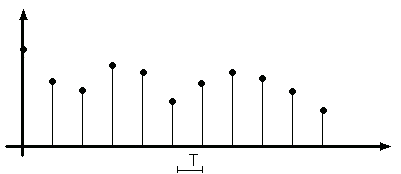
\includegraphics[width=0.7\linewidth]{tempo_discreto}
	\caption{ Segnale campionato nel tempo}
	\label{fig:tempodiscreto}
\end{figure}

\pagebreak
Quantizzazione: trasformiamo il codominio. Ha sempre perdita di informazione.\\

\begin{figure}[h]
	\centering
	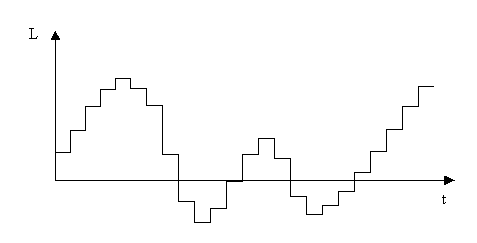
\includegraphics[width=0.7\linewidth]{quantizzato}
	\caption{ Segnale sinusoidale quantizzato nelle ampiezze}
	\label{fig:quantizzato}
\end{figure}

\textbf{Sistemi LTI}\\
Studiamo un tipo particolare di sistemi, che hanno due proprietà: linearità e tempo invarianza (L=lineari, TI=tempo invarianti).\\
- Linearità:\\
Se $ v_{1}=S(u_{1}) $ e $ v_{2}=S(u_{2})  $ 
allora $ S(\alpha u_{1} + \beta u_{2}) 
= \alpha S(u_{1}) + \beta S(u_{2})
= \alpha v_{1} + \beta v_{2} $ con $ \alpha , \beta \in C^{*} $ \\
Oppure grazie al \textbf{principio di sovrapposizione degli effetti} ( stabilisce che per un sistema dinamico lineare l'effetto di una somma di perturbazioni in ingresso è uguale alla somma degli effetti prodotti da ogni singola perturbazione): \\
$ S( \sum_{i=0}^n \alpha_i u_i ) 
=  \sum_{i=0}^n \alpha_i S( u_i )
$ \\
La linearità è dovuta alle equazioni differenziali, all'interno hanno la derivata prima che è essa stessa lineare.\\
- Tempo invariante:\\
 Significa che l'uscita non dipende esplicitamente dal tempo, cioè se un ingresso x(t) produce l'uscita y(t) allora per ogni ingresso traslato $x(t+ \delta )$ si ha un'uscita traslata dello stesso fattore $y(t+ \delta )$.\\
 
 $u(t+ t_0 ) \rightarrow v(t+ t_0 )$
 
\begin{figure}[h]
	\centering
	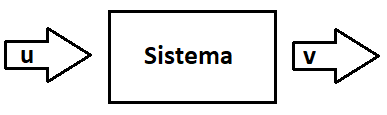
\includegraphics[width=0.7\linewidth]{sistema2}
	\caption{ Sistema generico }
	\label{fig:sistema2}
\end{figure}

\begin{figure}[h]
	\centering
	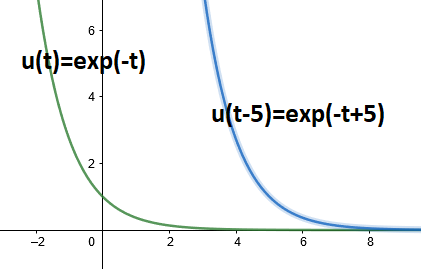
\includegraphics[width=0.7\linewidth]{esponenziale}
	\caption{ Esempio di tempo invariante }
	\label{fig:esponenziale}
\end{figure}


gniiiii
% TODO: eq diff a coefficienti costanti

\pagebreak

\section{ Ripasso sui numeri complessi }
\chapter{Segnali elementari}
\section{A tempo continuo}

\subsubsection{Segnali sinusoidali o fasori}

$ v(t)= Acos(wt+ \phi)$ con $t \in \mathbb{R}$.\\
Chiameremo: ampiezza $ A>0$, fase $ \phi $ (e se $ \phi > 0$ ho il segnale traslato a sinistra) , codominio $ [-A...A]$, periodo $ T = \frac{2 \pi}{w} $, pulsazione $w=\frac{2 \pi}{T} $ e frequenza $ f = \frac{1}{T}$ (NB: più grande è $T $ più piccola è f).\\
NB: $ w = 2 \pi f $ \\
NB: Come visto nell'Introduzione posso vedere il coseno come $  cosw = \frac{e^{jw} + e^{-jw}}{2}  $, quindi in questo caso $ cos(wt + \phi) = \frac{e^{jw+ \phi} + e^{-jw + \phi}}{2} $.\\

\subsubsection{Segnali sinusoidali modulati esponenzialmente}

$ v(t)= A e^{ \sigma t} cos(wt+ \phi)$ con $A>0$.\\
NB: In questo caso $T = \frac{2 \pi}{w} $ non è il periodo!\\

\begin{equation*}
v(t)=
\begin{cases} 
 \mbox{Converge, se } \sigma < 0 \rightarrow \mbox{ Il sistema è stabile }\\ 
 \mbox{Diverge, se } \sigma > 0 \rightarrow \mbox{ Il sistema è instabile}
\end{cases} 
\end{equation*}
Cioè $  \lim_{t \to \infty} v(t)=0$, solo se $ \sigma <0$.

\begin{figure}[h]
	\centering
	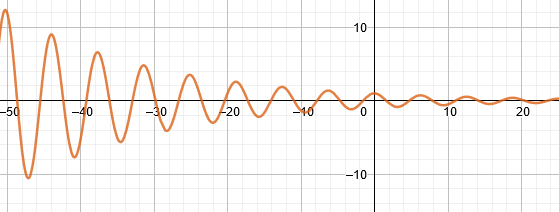
\includegraphics[scale=0.75]{immagini/segnSinNeg}
	\caption{ Andamento del segnale con $ \sigma <0$ }
	\label{fig: segnSinNeg}
\end{figure}

\pagebreak

\begin{figure}[h]
	\centering
	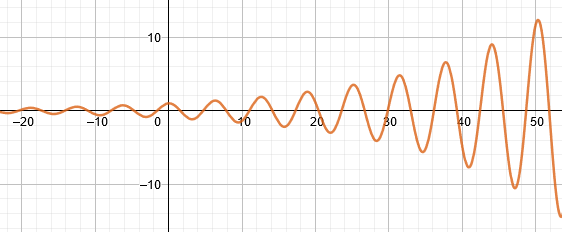
\includegraphics[scale=0.75]{immagini/segnSinPos}
	\caption{ Andamento del segnale con $ \sigma >0$ }
	\label{fig: segnSinPos}
\end{figure}

Come visto per il precedente segnale posso scrivere il coseno come $  cosw = \frac{e^{jw} + e^{-jw}}{2}  $.\\
In questo caso posso scrivere il segnale come:\\
$ v(t)= \frac{A}{2} e^{ \sigma t} e^{j(wt+ \phi)} + \frac{A}{2} e^{ \sigma t} e^{-j(wt+ \phi)}$\\
$= \frac{A}{2} e^{ \sigma t} e^{ jwt} e^{j \phi} + \frac{A}{2} e^{ \sigma t} e^{ -jwt} e^{-j \phi}$\\
$= \frac{A}{2} e^{j \phi} e^{( \sigma + jw) t} + \frac{A}{2} e^{-j \phi} e^{( \sigma - jw) t}$\\
Con $ s = \sigma + jw $ e $ \bar{s} = \sigma - jw $ posso scrivere che:\\
$= \frac{A}{2} e^{j \phi} e^{st} + \frac{A}{2} e^{-j \phi} e^{\bar{s} t}$\\
Cioè il segnale è la combinazione lineare di esponenziali complesse di cui una è il complesso conugato dell'altra.\\
 

\subsection{Funzioni generalizzate o distribuzioni}

Con distribuzioni intendiamo limiti di successioni di funzioni.\\

\subsubsection{Gradino unitario}
	
	\begin{equation*}
	\delta_{-1}(t)=
	\begin{cases} 
	1, \mbox{ se } t \geq 0\\ 
	0, \mbox{ se } t < 0
	\end{cases} 
	\end{equation*}
	
	\begin{figure}[h]
		\centering
		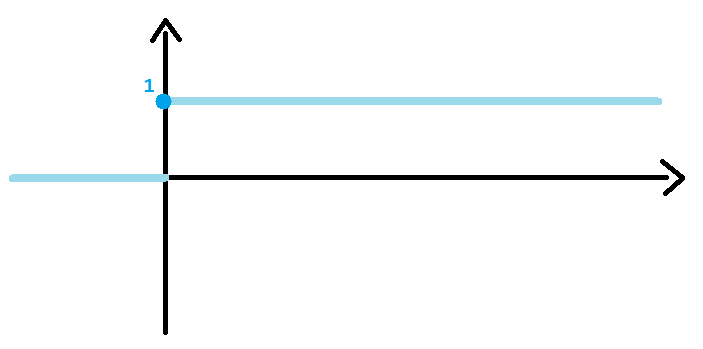
\includegraphics[scale=0.5]{immagini/gradinoContinuo}
		\caption{ Gradino unitario}
		\label{fig: gradinoContinuo}
	\end{figure}
	
	Proviamo ora a traslarla, con $ t_0 > 0$.\\
	
	Per avere un segnale in ritardo, dovrò traslare a destra e quindi sottraggo $t_0$.\\
	
	\begin{equation*}
	\delta_{-1}(t - t_0 )=
	\begin{cases} 
	1, \mbox{ se } t \geq t_0\\ 
	0, \mbox{ se } t < t_0
	\end{cases} 
	\end{equation*}
	
	\begin{figure}[h]
		\centering
		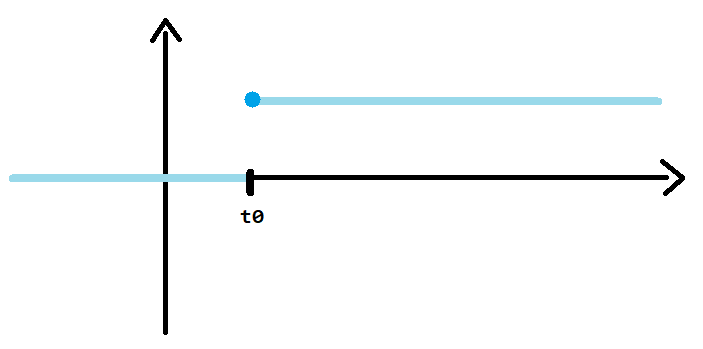
\includegraphics[scale=0.5]{immagini/gradinoContinuoMeno}
		\caption{ Gradino unitario $ \delta_{-1}(t - t_0 ) $ }
		\label{fig: gradinoContinuoMeno}
	\end{figure}
	
	Per avere un segnale in anticipo, dovrò traslare a sinistra e quindi sommo $t_0$.\\
	
	\begin{equation*}
	\delta_{-1}(t + t_0)=
	\begin{cases} 
	1, \mbox{ se } t \geq -t_0\\ 
	0, \mbox{ se } t < -t_0
	\end{cases} 
	\end{equation*}
	
	\begin{figure}[h]
		\centering
		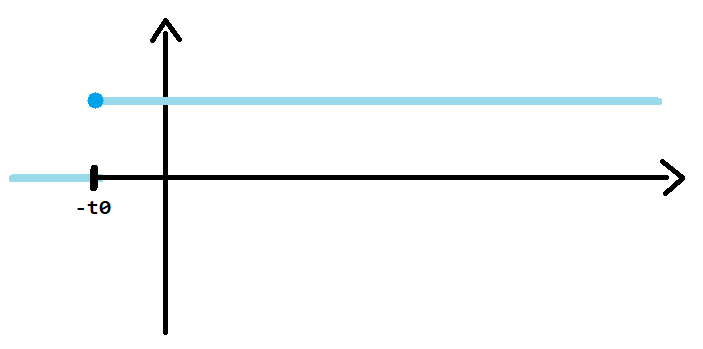
\includegraphics[scale=0.5]{immagini/gradinoContinuoPiu}
		\caption{ Gradino unitario $ \delta_{-1}(t + t_0 ) $ }
		\label{fig: gradinoContinuoPiu}
	\end{figure}
	
\pagebreak
	
	\textbf{COMANDO MATLAB:}\\
	
	\begin{figure}[h]
		\centering
		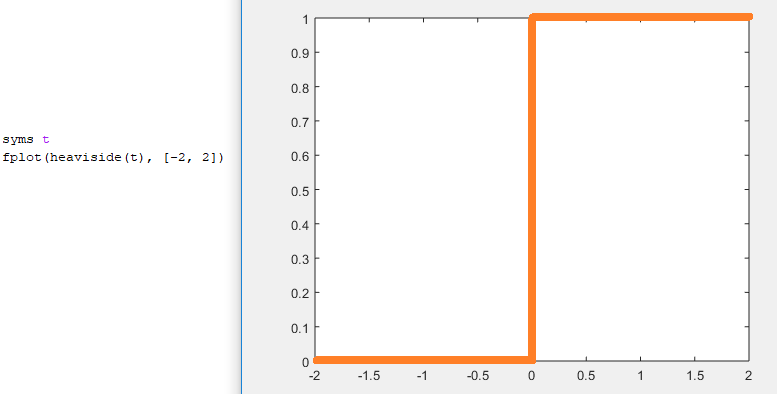
\includegraphics[scale=0.75]{immagini/comando2}
		\caption{ Il comando syms crea una variabile t, heaviside è la funzione per il gradino, fplot "plotta" cioè fa il grafico fra [-2...2]  }
		\label{fig: comando2}
	\end{figure}
	
	NB: da notare come la funzione gradino non è continua ma riusciremo comunque a derivarla.\\

\subsubsection{Funzione rettangolare di ampiezza e durata unitaria}
	
	\begin{equation*}
	\varPi(t)=
	\begin{cases} 
	1, \mbox{ se } -\frac{1}{2} \leq t \leq \frac{1}{2}\\ 
	0, \mbox{ altrimenti }
	\end{cases} 
	\end{equation*}
	
	\begin{figure}[h]
		\centering
		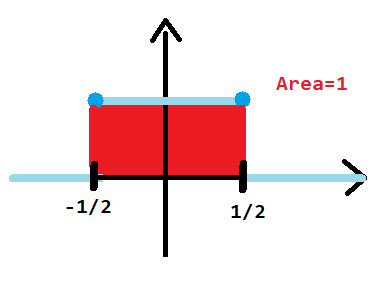
\includegraphics[scale=0.5]{immagini/rettangolo}
		\caption{ Funzione rettangolare di ampiezza e durata unitaria $ \varPi(t) $ }
		\label{fig: rettangolo}
	\end{figure}
	
	NB: è una combinazione lineare di due gradini:\\
	$ \varPi(t)= \delta_{-1}(t + \frac{1}{2}) - \delta_{-1}(t-\frac{1}{2}) $\\
	
	In generale il segnale sarà $ A \varPi( \frac{t-t_0}{T}) $, che mi dà una finestra di ampiezza A, durata T e centrata in $t_0$.\\
	
	\begin{equation*}
	A \varPi( \frac{t-t_0}{T})=
	\begin{cases} 
	A, \mbox{ se } -\frac{1}{2} \leq \frac{t-t_0}{T} \leq \frac{1}{2} \rightarrow -\frac{T}{2}+t_0 \leq t \leq \frac{T}{2}+ t_0 \\ 
	0, \mbox{ altrimenti }
	\end{cases} 
	\end{equation*}
	
	\begin{figure}[h]
		\centering
		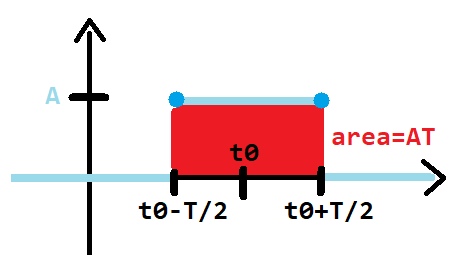
\includegraphics[scale=0.5]{immagini/rettangoloGenerale}
		\caption{ Funzione rettangolare in generale $ A \varPi( \frac{t-t_0}{T}) $ }
		\label{fig: rettangoloGenerale}
	\end{figure}


\subsubsection{Lambda: impulso triangolare di ampiezza e area unitaria}
	
	\begin{equation*}
	\varLambda(t)=
	\begin{cases} 
	0, \mbox{ se } t \leq -1\\ 
	1-|t|, \mbox{ se } -1 \leq t \leq 1\\ 
	0, \mbox{ se }  t > 1
	\end{cases} 
	\end{equation*}
	
	\begin{figure}[h]
		\centering
		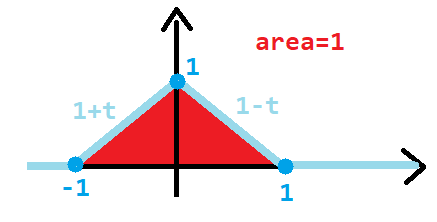
\includegraphics[scale=0.5]{immagini/lambda}
		\caption{ Funzione lambda $ \varLambda(t) $ }
		\label{fig: lambda}
	\end{figure}
	
	In generale il segnale sarà $ A \varLambda(t-t_0) $.\\
	
	\begin{equation*}
	A \varLambda( \frac{t-t_0}{T})=
	\begin{cases} 
	0, \mbox{ se } t \leq t_0-T\\ 
	\dfrac{A}{T}(|t|-t_0+T), \mbox{ se } t_0-T \leq t \leq t_0+T\\ 
	0, \mbox{ se }  t > t_0+T
	\end{cases} 
	\end{equation*}
	
	\begin{figure}[h]
		\centering
		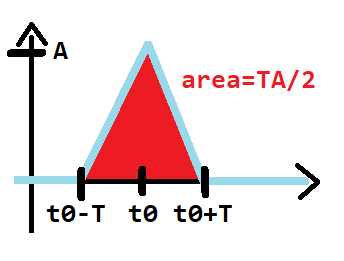
\includegraphics[scale=0.5]{immagini/lambdaGenerale}
		\caption{ Funzione lambda in generale $ A \varLambda( \frac{t-t_0}{T}) $ }
		\label{fig: lambdaGenerale}
	\end{figure}

\pagebreak

\subsubsection{Rampa unitaria}

	\begin{equation*}
	\delta_{-2}(t)=
	\begin{cases} 
	t, \mbox{ se } t \geq 0\\ 
	0, \mbox{ altrimenti }
	\end{cases} 
	\end{equation*}
	
	\begin{figure}[h]
		\centering
		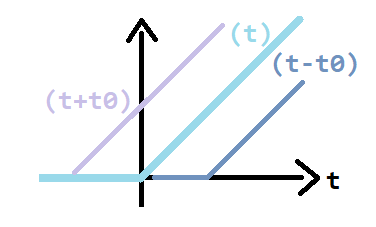
\includegraphics[scale=0.5]{immagini/rampaContinua}
		\caption{ Funzione rampa unitaria $\delta_{-2}(t) $ }
		\label{fig: rampaContinua}
	\end{figure}

\subsubsection{Riassunto: colleghiamo le distribuzioni}

	Notiamo che $ \delta_{-2}(t) = \int_{ -\infty}^{t} \delta_{-1}(\tau)  \, d \tau  $, sappiamo anche che per $ \tau <0 $ abbiamo $ \delta_{-1}(\tau) = 0 $ quindi $ \int_{ 0}^{t} \delta_{-1}(\tau)  \, d \tau $. Da 0 a t, ho $ \delta_{-1}(\tau) = 1 $ allora $ \int_{ 0}^{t} 1  \, d \tau = [ \tau]_0^t  = t $. \\
	Quindi l'integrale del gradino darà la rampa e la derivata della rampa darà il gradino:\\
	$ \delta_{-1}(t) =   \frac{d }{dt}\delta_{-2}(t)  $\\
	
	NB i numeri vicino alla delta saranno:\\
	Impulso o Delta $ \rightarrow 0 $ (lo zero viene omesso)\\
	Funzione costante o gradino $\rightarrow -1 $\\
	Retta o rampa $ \rightarrow -2 $\\
	Parabola $ \rightarrow -3 $\\
	Quest'ultima infatti la possiamo scrivere come:\\
	$ \delta_{-3}(t) = \int_{ -\infty}^{t} \delta_{-2}(\tau) \, d \tau = \int_{ 0}^{t} \tau \, d \tau = \frac{t^2}{2}$ .\\
	
	\begin{equation*}
	\delta_{-3}(t)=
	\begin{cases} 
	\frac{t^2}{2}, \mbox{ se } t \geq 0\\ 
	0, \mbox{ altrimenti }
	\end{cases} 
	\end{equation*}
	
	$ \frac{t^2}{2} $ è proprio una parabola.\\
	Come visto prima $ \delta_{-2}(t) = \frac{d }{dt}\delta_{-3}(t) $.\\
	
	In generale, andando avanti a integrare avrò che:\\
	
	\begin{equation*}
	\delta_{-k}(t)=
	\begin{cases} 
	\frac{t^{k-1}}{ (k-1)! }, \mbox{ se } t \geq 0\\ 
	0, \mbox{ altrimenti }
	\end{cases} 
	\end{equation*}
	
	Avrò quindi una serie di polinomi sempre con un grado in più.\\
	
\pagebreak

	Riassumendo quindi avrò:\\
	
	\begin{figure}[h]
		\centering
		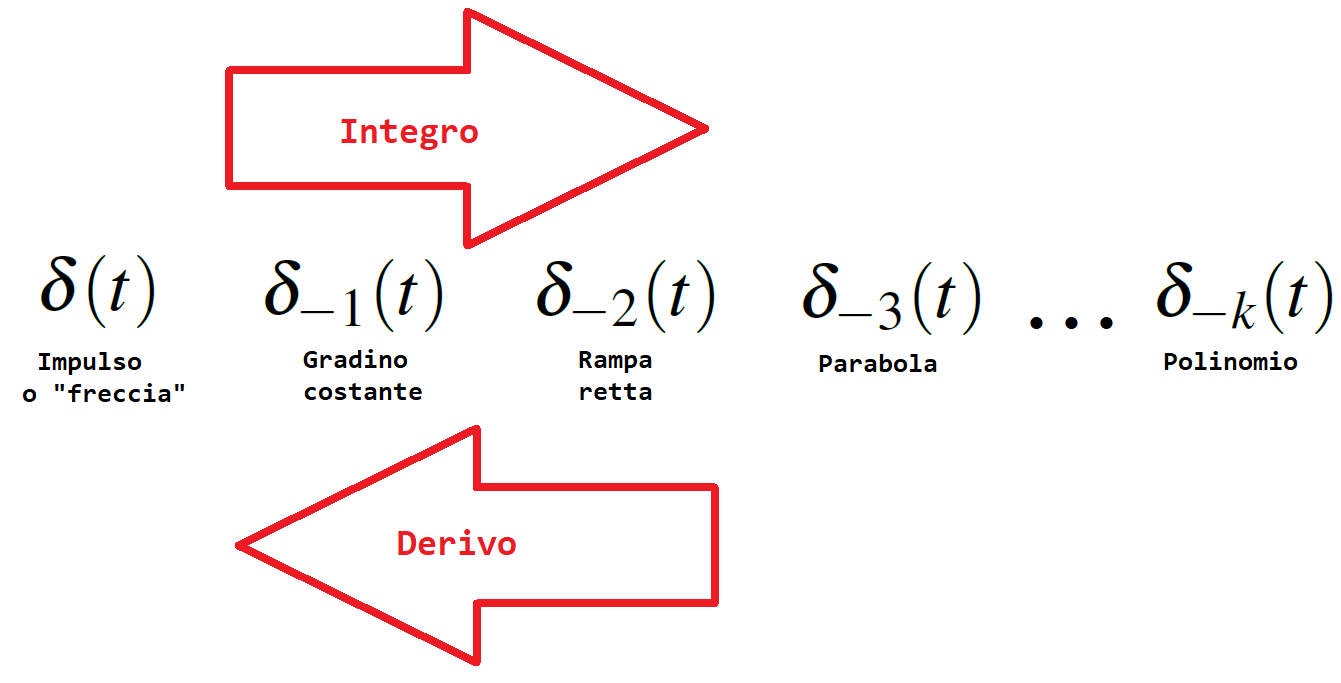
\includegraphics[scale=0.5]{immagini/riassuntoDistribuzioni}
		\caption{ Relazioni fra distribuzioni }
		\label{fig: riassuntoDistribuzioni}
	\end{figure} 

\subsubsection{Delta o impulso di Dirac}
	
	Abbiamo visto fino adesso funzioni generalizzate nel senso delle distribuzioni, cioè il limite di una serie di funzioni.\\
	Definiamo ora l'impulso di Dirac $ \delta(t)$ (sarebbe $ \delta_0 (t)$) come la derivata di $ \delta_{-1} (t)$ dal punto di vista delle distribuzioni (funzioni generealizzate, cioè limiti di successioni di funzioni).\\
	
	\textbf{OSS:} $ \delta_{-1} (t)$ come fuonzione standard non è continua e quindi non derivabile in $ t=0 $ ma nel senso delle distribuzioni si. Vogliamo vedere quindi $ \delta_{-1} (t)$ come il limite di $ \delta_{ \epsilon} (t)$.\\
	
	\begin{figure}[h]
		\centering
		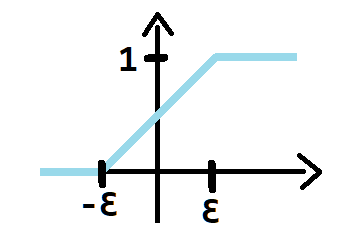
\includegraphics[scale=0.5]{immagini/deltaEpsilon}
		\caption{ $ \delta_{ \epsilon} (t)$ }
		\label{fig: deltaEpsilon}
	\end{figure}
	
	\begin{equation*}
	\delta_{ \epsilon}(t)=
	\begin{cases} 
	0, \mbox{ se } t < - \epsilon \\ 
	\frac{1}{2 \epsilon}t + \frac{1}{2}, \mbox{ se } - \epsilon \leq t < \epsilon\\
	1, \mbox{ se } t \geq \epsilon
	\end{cases} 
	\end{equation*}
	
	\begin{equation*}
	\delta_{-1}(t)= \lim_{ \epsilon \to 0} \delta_{\epsilon}(t)
	\end{equation*}

	Voglio ora una successione con $ n \in \mathbb{N} $ quindi sostituisco $ \epsilon = \frac{1}{n}$.\\
	Ottengo quindi $ \delta_{-1}(t)= \lim_{ n \to \infty} \delta_{\frac{1}{n}}(t) $ (ci sarà utile più avanti).\\
	
	Derivo ora $\delta_{-1}(t)= \lim_{ \epsilon \to 0} \delta_{\epsilon}(t) $: la parte a sinistra è facile da derivare perchè da prima so che $ \delta (t) = \frac{d}{dt} \delta_{-1}(t) $ mentre la parte a destra la dovremo fare per tratti (vedi com'è $ \delta_{\epsilon}(t) $ e lascia stare il limite).\\
	Ci verrà fuori che:
	\begin{equation*}
	\delta(t)= \lim_{ \epsilon \to 0} \frac{1}{2 \epsilon}  \varPi_{\epsilon}(\frac{t}{2 \epsilon})
	\end{equation*}
	
	\begin{figure}[h]
		\centering
		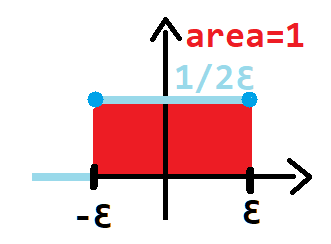
\includegraphics[scale=0.5]{immagini/rettangoloEpsilon}
		\caption{ $ \frac{1}{2 \epsilon}  \varPi_{\epsilon}(\frac{t}{2 \epsilon}) $ }
		\label{fig: rettangoloEpsilon}
	\end{figure}

	\textbf{OSS:} $ \forall \epsilon$, l'area è $\dfrac{1}{2 \epsilon} 2 \epsilon= 1 $ quindi l'area: è indipendente da $ \epsilon$, è costante e non cambia al variare di $ \epsilon $.\\
	
	\textbf{OSS:} per $ \epsilon \rightarrow 0 $ con $ \epsilon > 0 $, ho che $\dfrac{1}{2 \epsilon} \rightarrow \infty $ quindi l'area è sempre 1 ma l'ampiezza tende a $ + \infty $.\\
	
	\textbf{OSS:} $  \int_{ -\infty}^{ \infty} \delta(t)  \, dt = 1   $.\\
	
	\begin{figure}[h]
		\centering
		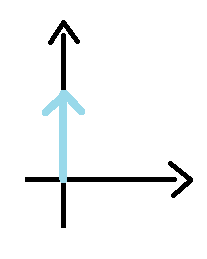
\includegraphics[scale=0.5]{immagini/delta}
		\caption{ Impulso di Dirac }
		\label{fig: delta}
	\end{figure}
	
	\textbf{NB:} può essere definita anche come il limite della seguente successione di funzioni:\\
	\begin{equation*}
	\forall n \in \mathbb{N} f_n(t)=
	\begin{cases} 
	\frac{n}{2}, \mbox{ se } -\frac{1}{n}\leq t \leq \frac{1}{n}\\
	0, \mbox{ altrimenti }
	\end{cases} 
	\end{equation*}
	
\pagebreak

	\begin{figure}[h]
		\centering
		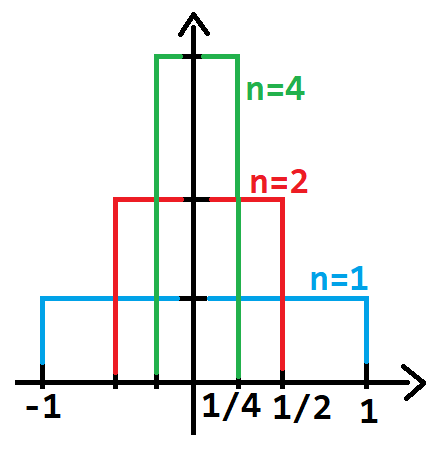
\includegraphics[scale=0.5]{immagini/deltaSuccessione}
		\caption{ $ f_n(t) $ }
		\label{fig: deltaSuccessione}
	\end{figure}

	Il limite quindi sarà:\\
	\begin{equation*}
	\lim_{ n \rightarrow \infty} f_n(t) = \delta(t) 
	\end{equation*}

\subsubsection{Proprietà dell'impulso}

	\textbf{1. } $\forall t \in \mathbb{R} \setminus $ \{ $ 0 $ \} cioè per $ t \neq 0 $ ho $ \delta(t)=0 $. \\
	
	\textbf{2. } (con O intendiamo l'origine)
	
	\begin{equation*}
	\int_{ a}^{ b} \delta( \tau)  \, d\tau =
	\begin{cases} 
	1, \mbox{ se } O \in (a...b)\\
	0, \mbox{ se } O \notin (a...b)
	\end{cases} 
	\end{equation*}
	
	\textbf{3. } Ho che $ \delta(t)=\delta(-t) $, quindi $ \delta(t) $ è pari.\\
	
	\textbf{4. Proprietà del campionamento}\\
	Se $ v(t) $ è continua in $ t_0 $ allora $ \forall t \in \mathbb{R}$:
	\begin{equation*}
	v(t) \delta (t-t_0) = v(t_0) \delta (t-t_0)
	\end{equation*}
	
	%TODO: da questo disegno in poi è tutto misterioso
	\begin{figure}[h]
		\centering
		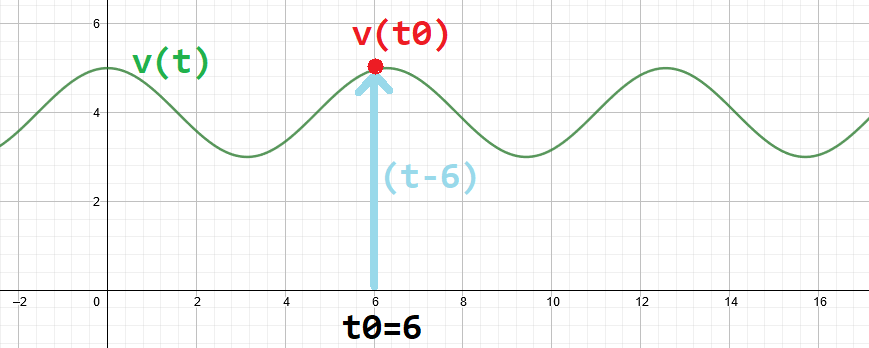
\includegraphics[scale=0.5]{immagini/campionamento}
		\caption{ Proprietà del campionamento }
		\label{fig: campionamento}
	\end{figure}

	\begin{equation*}
	v(t_0) = \int_{ - \infty}^{ \infty} v(t_0) \delta( \tau -t_0)  \, d\tau
	\end{equation*}
	
	\textbf{Conseguenze: }\\
	
	\textbf{1. } Per $ t=0 $ avrò che $ v(t) \delta (t) = v(t_0) \delta (t) $.\\
	
	\textbf{2. } Integriamo $ v(t) \delta (t-t_0) = v(t_0) \delta (t-t_0) $ verrà fuori che:\\
	$ \int_{ - \infty}^{ \infty} v( \tau ) \delta( \tau -t_0)  \, d\tau = \int_{ - \infty}^{ \infty} v( t_0 ) \delta( \tau -t_0)  \, d\tau$\\
	Di questa equazione posso rielaborare la parte destra considerando che $ v(t_0)$ non dipende da $ \tau $ e l'integrale di $ \delta (t-t_0) $ è 1. Quindi viene che:\\
	$ \int_{ - \infty}^{ \infty} v( \tau ) \delta( \tau -t_0)  \, d\tau = v(t_0)$\\
	
	\textbf{ $ \Rightarrow $ Proprietà di riproducibilità dell'impulso }\\
	%TODO: mi sa che qui c'è un errore, guarda bene i tuoi appunti
	Se $ v(t)$ è continua per $ \forall t \in \mathbb{R} $\\
	allora
	\begin{equation*}
	v(t) = \int_{ - \infty}^{ \infty} v( t ) \delta( \tau -t)  \, d \tau
	\end{equation*}
	\textbf{NB:} invece che $ t_0$ ho messo t perchè lo voglio generico avendo v(t) continua.\\
	
	\begin{proof}[Dim]
		Parto con un arteficio (da prendere così come ce l'ha dato il prof): $ v(t)=v(t_0)+( v(t) - v(t_0) )$\\
		Moltiplico da entrambe le parti per $ \delta (t-t_0)$:\\
		$ v(t) \delta (t-t_0) =v(t_0) \delta (t-t_0) +( v(t) - v(t_0) ) \delta (t-t_0) $\\
		Cambio t con $ \tau $ e integro:\\
		$ \int_{ - \infty}^{ \infty} v(\tau) \delta (\tau-t_0) \, d\tau 
		= \int_{ - \infty}^{ \infty} v(t_0) \delta (\tau-t_0) \, d\tau 
		+ \int_{ - \infty}^{ \infty} ( v(\tau) - v(t_0) ) \delta (\tau-t_0)\, d\tau $\\
		Qui devo fare varie considerazioni:\\
		1. Nel secondo integrale $ v(t_0) $ non dipende da $ \tau $ quindi posso portarlo fuori dall'integrale. \\
		2. Sempre nel secondo integrale, l'integrale di $ \delta (\tau-t_0) $ dà 1.\\
		3. Nel terzo integrale:\\
		Se ho $ \tau = t $ allora $ ( v(\tau) - v(t_0) ) = 0 $. \\
		Se ho $ \tau \neq t $ allora $ \delta (\tau-t_0) = 0 $. \\
		Allora il terzo integrale scompare.\\
		Quindi in fine avrò trovato che:\\
		$ \int_{ - \infty}^{ \infty} v(\tau) \delta (\tau-t_0) \, d\tau = v(t_0) $\\
		Questo vale per $ \forall t_0 $ per cui v(t) è continua (rendo quindi $t_0$ generica mettendo al suo posto t).\\ Quindi posso scrivere che:\\
		$ v(t) = \int_{ - \infty}^{ \infty} v(\tau) \delta (\tau-t) \, d\tau$
	\end{proof}

\subsubsection{Impulso centrato in $t_0$ e di area A: $ A \delta (t-t_0)$}

	\begin{figure}[h]
		\centering
		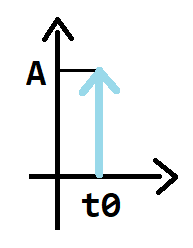
\includegraphics[scale=0.5]{immagini/deltaGenerica}
		\caption{ $ A \delta (t-t_0)$ }
		\label{fig: deltaGenerica}
	\end{figure}

\pagebreak

	\textbf{MATLAB}\\

	\begin{figure}[h]
		\centering
		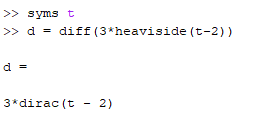
\includegraphics{immagini/comando3}
		\caption{Il comando syms mi crea una variabile t, diff mi fà la derivata di heaviside cioè il gradino. Come risultato ho dirac cioè proprio l'impulso.  }
		\label{fig: comando3}
	\end{figure}

\section{A tempo discreto}

Un segnale a tempo discreto è così definito (useremo k al posto di t per distinguerli):\\
$ v(k): \mathbb{Z} \rightarrow \mathbb{R} $

\subsubsection{Impulso discreto unitario (impulso di Kronecker)}

	\begin{equation*}
	\delta(k)=
	\begin{cases} 
	1, \mbox{ se } k=0 \\
	0, \mbox{ se } k \neq 0
	\end{cases} 
	\end{equation*}

	\begin{figure}[h]
	\centering
	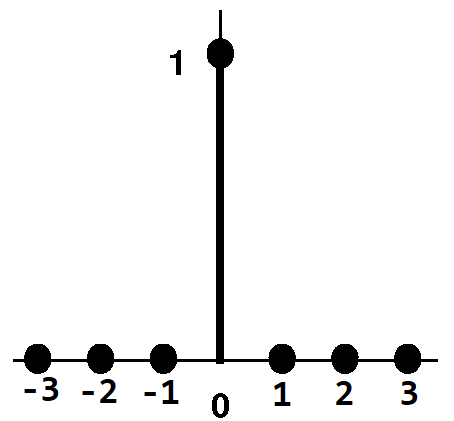
\includegraphics[scale=0.5]{immagini/impulsoDiscreto}
	\caption{ $ \delta(k)$ }
	\label{fig: impulsoDiscreto}
	\end{figure}

\subsubsection{Gradino discreto}

	\begin{equation*}
	\delta_{-1}(k)=
	\begin{cases} 
	1, \mbox{ se } k \geq 0 \\
	0, \mbox{ se } k < 0
	\end{cases} 
	\end{equation*}

\pagebreak
	
	\begin{figure}[h]
		\centering
		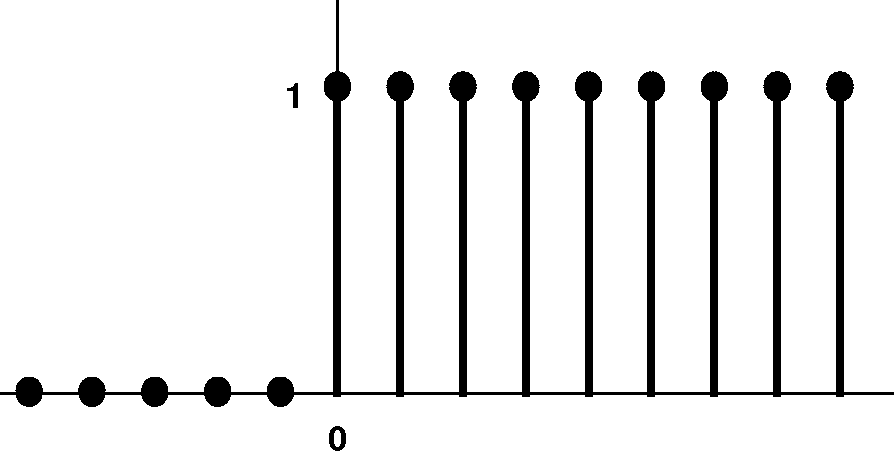
\includegraphics[scale=0.5]{immagini/gradino}
		\caption{ $ \delta_{-1}(k)$ }
		\label{fig: gradino}
	\end{figure}

	\textbf{OSS:}\\
	Se prendo $ k=-1 $, avrò $ \delta_{-1}(-1) = 0 $.\\
	Se prendo $ k=0 $, avrò $ \delta_{-1}(0) = \delta(0) = 1 $.\\
	Se prendo $ k=1 $, avrò $ \delta_{-1}(1) = \delta(0) = 1 $.\\
	
	%TODO: non ho capito
	\begin{equation*}
	\delta_{-1}(k)= \sum_{i=-\infty}^{k} \delta(i)
	\end{equation*}

\subsubsection{Rampa discreta}

	\begin{equation*}
	\delta_{-2}(k)=
	\begin{cases} 
	k, \mbox{ se } k \geq 0 \\
	0, \mbox{ se } k < 0
	\end{cases} 
	\end{equation*}
	
	\begin{figure}[h]
		\centering
		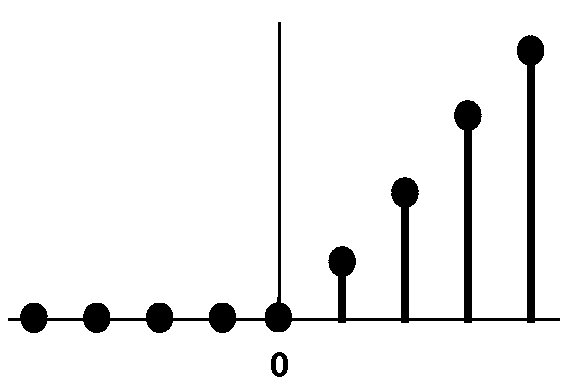
\includegraphics[scale=0.5]{immagini/rampaDiscreta}
		\caption{ $ \delta_{-2}(k)$ }
		\label{fig: rampaDiscreta}
	\end{figure}
	
	\textbf{OSS:}\\
	$ \delta_{-2}(0) = \sum_{i=-\infty}^{-1} \delta_{-1}(i) =0 $\\
	$ \delta_{-2}(1) = \sum_{i=-\infty}^{0} \delta_{-1}(i) = \delta_{-1}(0) $\\
	$ \delta_{-2}(2) = \sum_{i=-\infty}^{1} \delta_{-1}(i) = \delta_{-1}(0) + \delta_{-1}(1) $\\
	
	Si deduce quindi che:\\
	\begin{equation*}
	\delta_{-2}(k)= \sum_{i=-\infty}^{k-1} \delta_{-1}(i)
	\end{equation*}
	
	Ma allora questo significa che:\\
	\begin{equation*}
	\delta_{-2}(k)= \sum_{i=-\infty}^{ \infty} \sum_{j=-\infty}^{k-1} \delta(j)
	\end{equation*}
	
	Se $ k=0 $, allora $ \delta_{-2}(0) =0  $\\
	Se $ k=1 $, allora $ \delta_{-2}(1) = \delta_{-1}(0) = \delta(0) = 1  $\\
	Se $ k=2 $, allora $ \delta_{-2}(2) = \delta_{-1}(0) + \delta_{-1}(1) = \delta(0) + \delta(0) + \delta(1) = 1+1+0=2  $\\
	
	\textbf{Problema del campionamento ma in modo discreto }\\
	
	\begin{figure}[h]
		\centering
		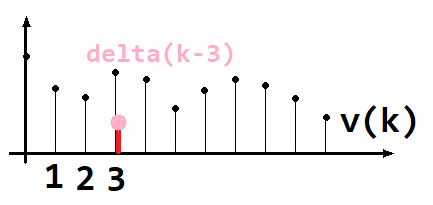
\includegraphics[scale=0.5]{immagini/campionamentoDiscreto}
		\caption{ Segnale a tempo discreto, $\delta(i-3)$ è l'impulso traslato in 3}
		\label{fig: campionamentoDiscreto}
	\end{figure}
	
	Il segnale v(k) ora è discreto (successione, $ k \in \mathbb{Z}$).\\
	Possiamo scrivere il segnale come:\\
	\begin{equation*}
	v(k)= \sum_{i=-\infty}^{ \infty} v(i) \delta(i-k)
	\end{equation*}
	
	In un determinato punto $ k=3$ sarà:\\
	\begin{equation*}
	v(3)= \sum_{i=-\infty}^{ \infty} v(i) \delta(i-3)
	\end{equation*}
	Tutti i termini della sommatoria saranno 0 a parte in 3.\\
	$ ...+0+0+0+ v(3) \delta(3-3)+0+0+0+...= v(3) \delta(0) = v(3)1 = v(3)$

\subsubsection{Successioni esponenziali}

	L'analogo segnale discreto è:
	\begin{equation*}
	v(k)= Ae^{j \phi} \lambda^k
	\end{equation*}
	con $ k \in \mathbb{Z} $, l'ampiezza $ A \in \mathbb{R}_+ $, $ \phi \in \mathbb{R} $ e $ \lambda \in \mathbb{C}$.\\
	
	Ricordiamo che $ \lambda $ essendo un numero complesso posso scriverlo anche come:\\
	 $ \rho ( cos\theta + j sen\theta) = \rho e^{j \theta} $\\
	Il segnale quindi diventerà:\\
	$ v(k)= Ae^{j \theta} \lambda^k = Ae^{j \theta} \rho^{k} e^{j \theta k} = Ae^{j \theta} e^{ (ln(\rho)+j\theta) k} $\\
	\textbf{NB:} nell'ultimo passaggio ho usato $ \rho = e^{ln(\rho)}$.\\
	\textbf{OSS:} v(k) può essere visto come la versione campionata (con periodo di campionamento unitario) del segnale esponenziale continuo.\\
	$ v(t) = Ae^{j \theta} e^{ ut} $ dove $ u=ln( \rho)+j \theta $.\\
	

\subsubsection{Successioni sinusoidali}

	L'analogo segnale discreto è:
	\begin{equation*}
	v(k)= Acos( \theta k + \phi)
	\end{equation*}
	con l'ampiezza $ A>0 $, $ \theta $ è la pulsazione e $ \phi$ la fase.\\
	
	v(k) è periodico se e solo se $ \theta = \frac{2 \pi n}{N}$, dove $n \in \mathbb{N} $, cioè è un multiplo razionale di $ 2 \pi $.\\
	$ N>0 $ è i periodo.\\
	

\subsubsection{Successioni sinusoidali modulate esponenzialmente}

	L'analogo segnale discreto è:
	\begin{equation*}
	v(k)= A \rho^k cos( \theta k + \phi)
	\end{equation*}
	con $ A>0 $, $ \rho>0 $, $ \theta$ e $\phi \in \mathbb{R}$.\\
	
	v(k) non è periodico perchè ho un esponenziale, si dice che v(k) è pseudo-periodico perchè devo comunque guardare la frequenza del campionamento.











%\postdisplaypenalty =1000

\chapter{Sistemi a tempo continuo}

	\begin{definizione}
		\textbf{un sistema dinamico} è un modello matematico che rappresenta un oggetto con un numero finito di gradi di libertà che evolve nel tempo secondo  una legge deterministica
	\end{definizione}
	\subsubsection{Esempi semplici}
		\begin{nexample}
			Il pendolo è un esempio semplice di sistema che ha come input la gravità e come output la posizione x nel tempo.
			Questo sistema è stabile perchè il pendolo tende a tornare nella posizione di equilibrio.
			
			\begin{figure}[H]
				\centering
				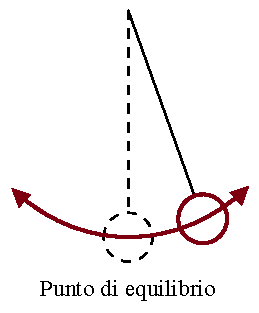
\includegraphics[scale=0.25]{immagini/cap3_Sistemi/pendolo}
				\caption{ Sistema semplice: pendolo. }
				\label{fig: pendolo}
			\end{figure}
			
			\begin{figure}[H]
				\centering
				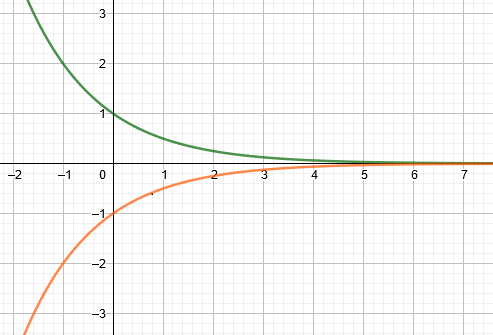
\includegraphics[scale=0.5]{immagini/esp3}
				\caption{ Grafico che descrive l'andamento nel tempo del pendolo, come si può vedere tende a zero infatti il sistema è in equilibrio. }
				\label{fig: esp3}
			\end{figure}
			
		\end{nexample}

%%\pagebreak

	\begin{nexample}
			Una palla che cade in una buca è un altro esempio di sistema stabile, l'input è sempre la gravità e la posizione x è l'output. 
		
		\begin{figure}[H]
			\centering
			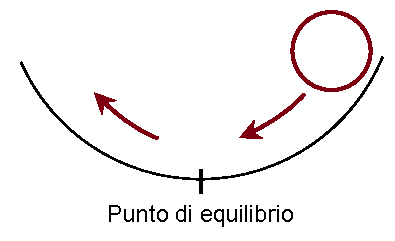
\includegraphics[scale=0.5]{immagini/cap3_Sistemi/pallaBuca}
			\caption{ Sistema semplice: palla che cade in una buca. }
			\label{fig: pallaBuca}
		\end{figure}
		
		\begin{figure}[H]
			\centering
			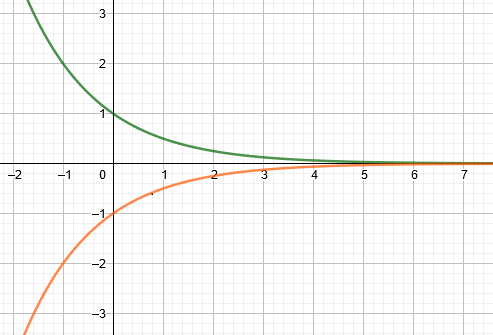
\includegraphics[scale=0.5]{immagini/esp3}
			\caption{ Grafico che descrive l'andamento della palla, come si può vedere tende a zero infatti il sistema è in equilibrio. }
			\label{fig: esp3}
		\end{figure}
	\end{nexample}
	
	\begin{nexample}
			Una palla che scivola da una collina è un esempio di sistema instabile, l'input è sempre la gravità e l'output è la velocità.
	
		\begin{figure}[H]
			\centering
			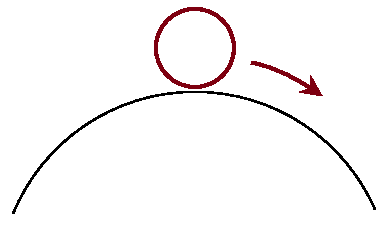
\includegraphics[scale=0.5]{immagini/cap3_Sistemi/pallaScivola}
			\caption{ Sistema semplice: pendolo. }
			\label{fig: pallaScivola}
		\end{figure}
	
		\begin{figure}[H]
			\centering
			\includegraphics[scale=0.5]{immagini/cap3_Sistemi/esp1Causale}
			\caption{ Grafico che descrive l'andamento della velocità di una palla che scivola, come si vede la velocità continuerà ad aumentare. }
			\label{fig: esp1Causale}
		\end{figure}

	\end{nexample}
%%\pagebreak

%%%%%%%%%%%%%%%%%%%%%%%%%%%%%
%% Proprietà dei sistemi a tempo continuo
%%%%%%%%%%%%%%%%%%%%%%%%%%%%%

\section{Proprietà dei sistemi a tempo continuo}
	
	\subsection{Proprietà intrinseche: linearità, tempo invarianza e causalità}
	Con proprietà intrinseche intendiamo che i nostri sistemi per forza devono soddisfare queste proprietà.
		
		\subsubsection{Linearità}\label{sist_prop_Lin} 
		%TODO Aggiungere descrizione 
		%TODO immaigne: fare la formula come sistema a blocchi?
			\[
			\alpha u_1+\beta u_1 \overset{\text{sistema}}{\longmapsto} \alpha v_1+\beta v_2
			\]
			dove $ u_1 \overset{\text{sistema}}{\longmapsto} v_1$ e $u_2\overset{\text{sistema}}{\longmapsto} v_2$
			
		\subsubsection{Tempo invarianza} \label{sist_prop_TIn}
		%TODO Aggiungere descrizione 
		%TODO immaigne: fare la formula come sistema a blocchi?
			\[
			u(t-\tau) \overset{\text{sistema}}{\longmapsto} v(t-\tau)
			\]
			Se traslo nel tempo un segnale allora il segnale in uscita sarà traslato nel tempo della stessa quantità.
			
			\begin{definizione}
				I sistemi che soddisfano la linearità e la tempo invarianza li chiameremo sistemi LTI.
			\end{definizione}
		
		\subsubsection{Causalità (o non anticipatorio):} \label{sist_prop_cau}
			
			Con causalità si intende che l'effetto non precede la causa (la causa anticipa l'effetto).
			
			\begin{osservazione}
				Ci sarà sempre un istante iniziale $t_0$ a partire da cui studieremo il sistema.
			\end{osservazione}
			\[
				\exists \,t_0 \in \R \text{ tale che } u(t)=0 \text{ per } t<t_0
				\text{, allora } v(t)=0 \text{ per } t<t_0
			\]		
			Grazie alla tempo invarianza e alla causalità posso prendere per convenzione $ t_0 = 0$, cioè l'origine dell'evento.
			
%\pagebreak
		
			\begin{figure}[H]
				\centering
				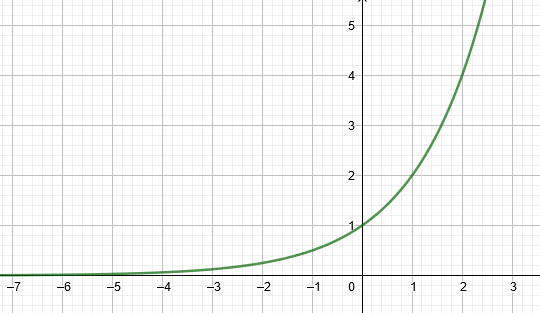
\includegraphics[scale=0.5]{immagini/esp1}
				\caption{ Sistema non causale. }
				\label{fig: esp1}
			\end{figure}
			
			\begin{figure}[H]
				\centering
				\includegraphics[scale=0.5]{immagini/cap3_Sistemi/esp1Causale}
				\caption{ Sistema causale con $ t_0 = 0$. }
				\label{fig: esp1Causale}
			\end{figure}
	
	\subsection{Proprietà richieste: stabilità BIBO e stabilità asintotica}

		\subsubsection{Stabilità BIBO (bounded input bounded output)}\label{sist_prop_BIBOstab}
			
			Se l'entrate è limitata allora anche l'uscita sarà limitata (per sistemi causali).
			
			Scriviamo l'ingresso limitato come:
			\[
				\forall t \in [t_0, + \infty) \subseteq \R\text{, } \exists \, M_u >0 \text{ tale che } \lvert u(t) \rvert < M_u	
			\]
			
			Allora l'uscita limitata sarà:
				\[
			\exists \, M_v > 0 \text{ tale che } \forall t \in [t_0, + \infty) \text{, } \lvert v(t) \rvert < M_v
			\]
			%TODO aggiungere disegno
			
		\subsubsection{Stabilità asintotica}


			Se $\exists \, t_0 \text{ tale che } u(t)=0 \text{, } \forall t \ge t_0 \text{ allora } \lim_{t \to +\infty} v(t)=0$.\\
			In parole povere, in assenza di input l'output converge a zero asintoticamente: $\lim_{t \to \infty} v(t)=0$.
			
			\begin{NB}				
			La stabilità asintotica è più forte della BIBO, ovvero se trovo che un sistema è stabile asintoticamente so per certo che è anche BIBO stabile (non vale il contrario!).
			\end{NB}
			%TODO: aggiungere immagini?

%%%%%%%%%%%%%%%%%%%%%%%%%%%%%
%% Modelli
%%%%%%%%%%%%%%%%%%%%%%%%%%%%%
	
\section{Modelli descritti da equazioni differenziali}

\subsection{Esempi pratici}
\begin{nexample}
	Circuito elettrico
	
		\begin{figure}[H]
			\centering
			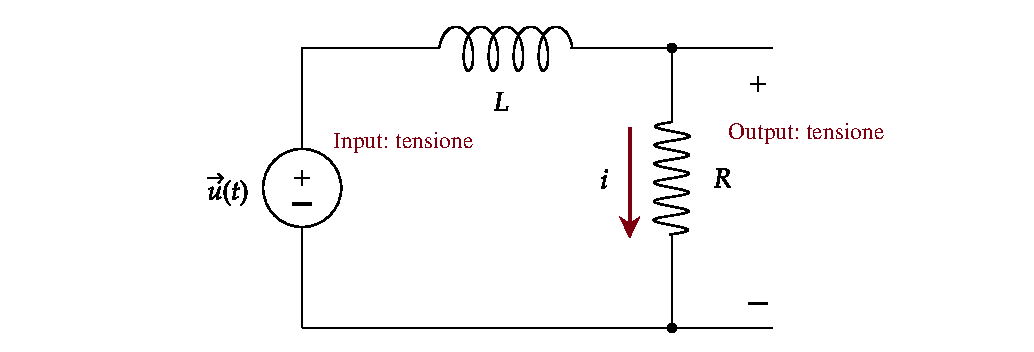
\includegraphics[scale=0.75]{immagini/cap3_Sistemi/circuito_RLC}
			\caption{ Circuito RLC. }
			\label{fig: circuito_RLC}
		\end{figure}
	 	In questo ambito L è l'induttanza (misurata in Henry) e R è la resistenza (misurata in Ohm). 
 	
	 	Per la legge di Kirchhoff trovo che: 
	 	\[ u(t) = L \frac{di(t)}{dt} + R i(t) \quad \text{e} \quad v(t) = R i(t) \]
	 	
	 	Allora avrò che $ \frac{L}{R} \frac{dv(t)}{dt} + v(t) = u(t)$ che posso riscrivere come:
	 	  \[ \frac{dv(t)}{dt} + \frac{R}{L} v(t) = \frac{R}{L} u(t) \]
	 	  
	 	Ho così modellato il sistema con un'equazione differenziale.
\end{nexample}

\begin{nexample}
	\label{es_mms}
	Sistema massa-molla-smorzatore 
	
		\begin{figure}[H]
			\centering
			
\includegraphics{immagini/cap3_Sistemi/massa_molla_smorzatore}
			\caption{ Sistema massa-molla-smorzatore. }
			\label{fig: massa_molla_smorzatore}
		\end{figure}
		
		In questo ambito Fk è la forza della molla (K costante elastica), Fd è la forza dello smorzatore (D costante di smorzamento), M è la massa, u(t) è la forza che applichiamo al sistema (l'input) e v(t) è lo spostamento nel tempo (l'output).
		
		\begin{NB}
			 v(t) è uno spostamento, non si intende una velocità! Quindi, solo in questo caso scriviamo: $ v(t) = x(t) $.
			Sapendo che $ F=ma $ e che $a= \frac{d^2 x(t)}{dt} $ abbiamo che:
			\[  M \frac{d^2 x(t)}{dt} = u(t) - F_d(t) - F_k(t) = u(t) - D \frac{d x(t)}{dt} - K x(t) \]
			con $ F_d $ e $ F_k $ forze opposte allo spostamento.
		\end{NB}
		
		Trovo anche qui una equazione differenziale che mi modella il sistema:
		\[  M x''(t) + D x'(t) + K x(t) = u(t) \]
		Sostituendo di nuovo avrò che:
		\[ M v''(t) + D v'(t) + K v(t) = u(t) \]
\end{nexample}


\subsection{Modelli SISO}

	In generale un modello SISO è descritto da un'equazione differenziale a coefficienti costanti di ordine $ n $.
	\begin{multline}
		a_n \frac{d^{(n)} v(t)}{dt^n} 
			+ a_{n-1} \frac{d^{(n-1)} v(t)}{dt^{n-1}} 
			+ \dots 
			+ a_1 \frac{dv(t)}{dt} 
			+ a_0\,v(t)\\
		= b_m \frac{d^{(m)} u(t)}{dt^m}
			+ b_{m-1} \frac{d^{(m-1)} u(t)}{dt^{m-1}} 
			+ \dots
			+ b_1 \frac{du(t)}{dt} 
			+ b_0\,u(t)
	\tag{2}\label{equation 2}
	\end{multline}
	con $ a_n, b_m \ne 0 $ ( Si ricorda che la parte a sinistra dell'uguale è l'output mentre quella a destra è l'input).
	
	Ricordiamo qui, per comodità, la prima equazione vista, cioè:
	\begin{equation*}
		\sum\limits_{i=0}^n a_{i} \frac{ d^{i} v }{ dt^{i}  } = \sum\limits_{i=0}^m b_{i} \frac{ d^{i} u }{ dt^{i}  }
		\tag{\ref{equation 1} rev.}
	\end{equation*}

	\begin{osservazione}
		Nei casi pratici, cioè in un sistema fisico, avrò che $n \ge m$.
	\end{osservazione}

	\begin{nexample}
		dall'esempio \ref{es_mms} di prima:
		 \[ M v''(t) + D v'(t) - K v(t) = u(u) \]
		quindi abbiamo che $ n = 2 $ e $ m = 0 $.
	\end{nexample}

	
	\begin{definizione}
		I sistemi in cui $n \ge m$ si chiamano \textbf{propri}.
		Se $n > m$ il sistema si chiamerà \textbf{strettamente proprio}.
	\end{definizione}
	
	\begin{osservazione}
		In generale l'uscita $v(t)$ del sistema (\ref{equation 1}) non è univoca.
		Se definiamo $n$ \textbf{condizioni iniziali} all'istante $t_0 = 0^-$ (per l'uscita $v$):
		\begin{equation}
			v(0^-) \,
			,\, \frac{dv(t)}{dt}\bigg\vert_{t=0^-} \,
			,\, \dots\,
			,\, \frac{d^{(n-1)}v(t)}{dt^{n-1}}\bigg\vert_{t=0^-}
			\tag{3}\label{equation 3}
		\end{equation}
		allora la soluzione di (\ref{equation 1}) è unica.
	\end{osservazione}
	
\subsection{Soluzione dei modelli SISO (evoluzione libera e forzata)}
	
	La soluzione dell'equazione (\ref{equation 1}) si ottiene come somma fra:
	\begin{itemize}
		\item una soluzione che dipende soltanto dalle condizioni iniziali (\ref{equation 3}) chiamata \textbf{evoluzione libera} con simbolo $v_l(t)$.
		\item una soluzione che dipende soltanto dall'ingresso $u(t)$ con condizioni iniziali tutte nulle, chiamata \textbf{ evoluzione forzata} con simbolo $v_f(t)$.
	\end{itemize}
	Avremo, cioè, che la soluzione dell'equazione (\ref{equation 1}) è:\\
	\[
	v(t) = v_l(t) + v_f(t)
	\]
	
\section{Evoluzione libera $ \rightarrow $ codizioni iniziali}
	L'evoluzione libera si ottiene dall'equazione dell'\textbf{omogenea associata}
	\begin{equation}
		a_n \frac{d^{(n)} v(t)}{dt^n} 
			+ a_{n-1} \frac{d^{(n-1)} v(t)}{dt^{n-1}} 
			+ \dots 
			+ a_1 \frac{dv(t)}{dt} 
			+ a_0\,v(t)
		= 0
		\tag{4}\label{equation 4}
	\end{equation}
	e le condizioni iniziali (\ref{equation 3}).
	
	Associamo a (\ref{equation 4}) l'\textbf{equazione caratteristica}:
	\begin{equation}
		a_n s^n 
		+ a_{n-1} s^{n-1}
		+ \dots
		+ a_1 s^1
		+ a_0 = 0
		\tag{5}\label{equation 5}
	\end{equation}
	con $a_n s^n + a_{n-1} s^{n-1} + \dots + a_1 s^1 + a_0 $ polinomio caratteristico.\\

	Sappiamo che per il toerema fondamentale dell'algebra, l'equazione (\ref{equation 5}) ha $r$ radici  distinte: $\lambda_1,\lambda_2, \dots, \lambda_r$ di molteplicità $\mu_1, \mu_2, \dots,\mu_r$ dove  $\mu_1 +\mu_2 + \dots + \mu_r = n$.
	
	La soluzione di (\ref{equation 4}) sarà:
	\begin{equation}
		v_\l(t)=  \sum_{i=1}^{r}\sum_{\l=0}^{\mu_i-1}c_{i,\l} \,e^{\lambda_it}\frac{t^\l}{\l!}
		\tag{6}\label{equation 6}
	\end{equation}
	con i coefficienti $c_{i,\l} $ che hanno indici $ i=\overline{1,r} $ e $ \l=\overline{o,\mu_{i-1}}$, $ \forall\mu_i \in \{\mu_1,\mu_2,\dots,\mu_r\} $. I coefficienti verranno determinati dalle condizioni iniziali (\ref{equation 3}).
		
	\begin{osservazione}
		Se $\mu_1 = \mu_2 = \dots = \mu_r = 1$ allora:
		\begin{equation*}
			v_l(t)=  \sum_{i=1}^{n}c_{i} \,e^{\lambda_it}
		\end{equation*}
		In cui mancano sia la seconda sommatoria sia $ \frac{t^\l}{\l!}$.
	\end{osservazione}
	
	\begin{definizione}
		$\displaystyle m(t) = e^{\lambda_i t} \frac{t^\l}{\l!} $ si chiama \textbf{modo elementare} del sistema.
	\end{definizione}
	\begin{nexample}
	L'equazione caratteristica è $ s^3 + 3 s^2 + 3s +1=0$
	
	Si ha che $ (s+1)^3=0$, avremo $ \lambda_{1} = -1$ con $ \mu_1=3 $. 
	Possiamo quindi scrivere la risposta libera come:
	\[ v_\l(t) =\sum_{i=1}^{r}\sum_{\l=0}^{\mu_i-1}c_{i,\l} \,e^{\lambda_it}\frac{t^\l}{\l!} \]
	Abbiamo, però, solo una radice quindi la prima sommatoria se ne va e rimane:
	 \[ v_\l(t) =\sum_{\l=0}^{3-1}c_{1,\l} \,e^{-1 t}\frac{t^\l}{\l!}  \]
	 \[ = c_{1,0} \, e^{-1t} + c_{1,1}\, e^{-1t} t + c_{1,2}\, e^{-1t} \frac{t^2}{2} \]
	\end{nexample}
	
	\begin{nexample}
	L'equazione caratteristica è $ (s+2)^2(s+1)^3=0 $
	
	Avrò quindi che $ \lambda_{1} = -2 $ con $ \mu_1=2 $ e $ \lambda_{2} = -1 $ con $ \mu_2=3 $.\\
	\[  v_\l(t) =\sum_{i=1}^{2}\sum_{\l=0}^{\mu_i-1}c_{i,\l} \,e^{\lambda_it}\frac{t^\l}{\l!} \]
	 \[ = c_{1,0}\, e^{-2t} + c_{1,1}\, e^{-2t} t + c_{2,0}\, e^{-t} + c_{2,1}\, e^{-t} t + c_{2,2}\, e^{-t} \frac{t^2}{2} \]
	\end{nexample}


	\begin{theorem}
		Dato un modo elementare $m(t) = e^{\lambda t} \frac{t^\l}{\l!} $ con $ \l \in \Z_+$, $ t \in \R$ e $ \lambda \in \C $.\\
		Abbiamo che:
		\begin{description}		
		\item[a)] $\Re( \lambda ) < 0 \Leftrightarrow  \lim_{t \to \infty} \, m(t) = 0 $.
		\item[b)] $\Re( \lambda ) \leq 0 \Leftrightarrow  m(t)$ limitato su $ [0, + \infty) $ e se $ Re( \lambda ) = 0 $ e $ \l=0$.
		\item[c)] in tutti gli altri casi ( cioè $ \Re( \lambda ) > 0 $ oppure $ \Re( \lambda ) = 0 $ e $ \l \neq 0$ ), $ \lim_{t \to \infty} m(t) = \infty $.
		\end{description}
	
		\begin{proof}[Dim]
		dimostriamo per casi.
		
		Sappiamo che $ \lambda \in \C$ quindi possiamo scriverlo anche come $ \lambda = \sigma + j \omega$ con $ \sigma = Re( \lambda)$.\\
		Possiamo quindi riscrivere il limite:
		 \[ \lim_{t \to \infty} m(t) = \lim_{t \to \infty} e^{\lambda t} \frac{t^\l}{\l!}= \lim_{t \to \infty} e^{(\sigma + j \omega ) t} \frac{t^\l}{\l!}= \lim_{t \to \infty} e^{\sigma t} e^{ j \omega t} \frac{t^\l}{\l!} \]
		\begin{description}	
		\item[c)] $ \sigma > 0$
		
		Allora $\displaystyle \lim_{t \to \infty} e^{\sigma t} e^{ j \omega t} \frac{t^\l}{\l!} = + \infty $ (il primo e il terzo tendono a $ \infty$, il secondo è limitato).
		Stessa cosa con $ \sigma = 0 $ e $ \l \neq 0 $ (il terzo tende a $ \infty$, il secondo è limitato, il primo tende a 1).
		
		\item[b)] $ \sigma > 0$ e $ \l =0$
		
		Allora $\displaystyle \lim_{t \to \infty} \frac{t^\l}{\l!} e^{\sigma t} e^{ j \omega t}$, il primo e il secondo tendono a 1, quindi possiamo scrivere il terzo argomento come $ \lim_{t \to \infty} ( \cos (\omega t) + j \sin (\omega t)) $.
		
		Il limite quindi non esiste ma è limitato tra -1 e 1.
		
		\item[a)] $ \sigma < 0$
		
		Allora $\displaystyle \lim_{t \to \infty} \frac{t^\l}{\l!} e^{\sigma t} e^{ j \omega t} = \lim_{t \to \infty} \frac{t^\l }{\l! e^{-\sigma t}}  e^{ j \omega t} = 0$ (la forma è indeterminata $\displaystyle \frac{\infty}{\infty}$, vince quello sotto).
	\end{description}	
		\end{proof}
	\end{theorem}

%%%%%%%%%%%%%%%%%%%%%%%%%%%%%
%% Stabilità asintotica
%%%%%%%%%%%%%%%%%%%%%%%%%%%%%

\section{Stabilità asintotica}
	
	Si studia la stabilità asintotica di sistemi descritti dall'equazione:
	\begin{equation*}
	\sum\limits_{i=0}^n a_{i} \frac{ d^{i} v }{ dt^{i}  } = \sum\limits_{i=0}^m b_{i} \frac{ d^{i} u }{ dt^{i}  }
	\tag{\ref{equation 1} rev.}
	\end{equation*}

	
	Dal teorema visto prima ne enunciamo un altro di maggiore importanza.
	
	\begin{theorem}
		il sistema (\ref{equation 1}) è asintoticamente stabile se per ogni scelta delle condizioni iniziali (\ref{equation 3}):
		\begin{equation*}
			\lim_{t \to \infty}v_\l(t)=0
			\Leftrightarrow\text{tutti i modi elementari } m(t)=e^{\lambda t}\frac{t^\l}{\l!}\text{ sono convergenti a $0$}
			\Leftrightarrow \Re(\lambda_i)<0,\forall i = \overline{1,r}
		\end{equation*}
	\end{theorem}
	\begin{nexample}
	Analizziamo la stabilità del circuito elettrico
	
	Abbiamo visto che il circuito elettrico RLC è modellato da:
	 \[ \frac{dv(t)}{dt} + \frac{R}{L} v(t) = \frac{R}{L} u(t) \]
	L'equazione caratteristica è $ s + \frac{R}{L}=0 $ con s numero complesso.
	Ho un'unica radice che risolve l'equazione ed è $ \lambda = - \frac{R}{L}$ con $ R > 0$ e $ L > 0$.
	
	$\Re(\lambda) = - \frac{R}{L}$ e noi vogliamo che sia negativa (dal teorema precedente). Visto che ho $ R > 0$ e $ L > 0$, allora il sistema sarà sempre stabile.
	\end{nexample}

	\begin{nexample}	
	Calcoliamo la risposta libera del sistema massa-molla-smorzatore.
	
	Abbiamo visto che questo sistema è modellato da:
	 \[ M v''(t) + D v'(t) - K v(t) = u(t) \]
	con $ M, D, K>0 $.
	
	L'equazione caratteristica è $ M s^2 + Ds + K=0 $ con s numero complesso.
	
	Le radici saranno $\displaystyle \lambda_{1,2} = \frac{-D\pm \sqrt{D^2 - 4KM}}{2M}$.
	\begin{itemize}
		\item Se $ \lambda_{1} \neq \lambda_{2} $ allora la risposta libera è $ v_\l(t) = C_{1,0}\, e^{\lambda_{1}t} + C_{2,0}\, e^{\lambda_{2}t}$.
		\item Se $ \lambda_{1} = \lambda_{2} $ allora la risposta libera è $ v_\l(t) = C_{1,0}\, e^{\lambda_{1}t} + C_{1,1}\, e^{\lambda_{1}t} $.
	\end{itemize}
	\end{nexample}


%%%%%%%%%%%%%%%%%%%%%%%%%%%%%
%% Convoluzione
%%%%%%%%%%%%%%%%%%%%%%%%%%%%%

\section{Convoluzione}
	
	\begin{definizione}
		Date due funzioni $v_1(t)$ e $v_2(t) $ con $ t\in\mathbb{R} $ definiamo il prodotto (o integrale) di \textbf{convoluzione} come:
		\begin{equation*}
			(v_1 * v_2)(t_0) 
			= \int_{-\infty}^{\infty}v_1(\tau)v_2(t_0 - \tau)\d\tau 
			= \int_{-\infty}^{\infty}v_1(t_0 - \tau)v_2(\tau )\d\tau
		\end{equation*}
		con $t_0 $ fissato.
	\end{definizione}
		
	Proprietà della convoluzione:
		\begin{enumerate}
			\item $v_1 * v_2 = v_2 * v_1 $ (commutatività)
			\item $(v_1 * v_2) * v_3  = v_1 * (v_2 * v_3) $ (associatività)
			\item $v_1 * (v_2 + v_3)  = v_1 * v_2 + v_1 * v_3$ (distributività rispetto alla somma)
		\end{enumerate}
		Queste proprietà sono immediate, per dimostrarle sostituisco con gli integrali.
	
	\begin{osservazione}
		\textbf{Proprietà di riproducibilità dell'impulso}
		
		L'elemento neutro della convoluzione è $ \delta(t)$.
		\[ (v *\delta)(t)\overset{def}{=} \int_{-\infty}^{\infty}v(\tau)\delta(t - \tau)\d\tau = v(t) \]
	\end{osservazione}
	
	Dimostrazione fatta con il sistema a box (guarda gli appunti). %TODO: riferimento a cosa?
	%TODO: se hai voglia fallo
		
%%%%%%%%%%%%%%%%%%%%%%%%%%%%%
%% Risposta impulsiva
%%%%%%%%%%%%%%%%%%%%%%%%%%%%%

\section{Risposta impulsiva}
	
	\begin{definizione}
		Dato un sistema descritto dall'equazione (\ref{equation 1}), inizialmente a riposo, definiamo la \textbf{risposta impulsiva} l'uscita del sistema in corrispondenza dell'impulso unitario $\delta (t)$ in ingresso. La indichiamo con $h(t)$.
	\end{definizione}
	
	\textbf{In parole semplici: }
	\begin{enumerate}
	\item Posso calcolare la risposta impulsiva $ h(t) $  definita come l'uscita con ingresso un impulso $\delta(t)$.
	\item Grazie ad esso posso trovare l'uscita di un sistema facendo la convoluzione fra l'ingresso e $ h(t) $.
	\end{enumerate}

	\textbf{In dettaglio: } 
		
	Tenendo conto che $h(t)=0$ per $t<0$ (causalità) avremo:
	\begin{equation*}
	v(t)= \int_{0^-}^{\infty}h(\tau)u(t - \tau)\d\tau 
	= \int_{-\infty}^{t^+}h(t - \tau)u(\tau)\d\tau
	\end{equation*}
	Tutto ciò è dovuto sostituiendo:  $t-\tau = s \Rightarrow d\tau = - ds 
	\qquad \tau = 0^-  \Rightarrow s = t^+ 
	\qquad \tau=\infty \Rightarrow s = -\infty$
	
	Ora è possibile cambiare gli estremi dell'integrale con un cambio di segno.
	\[
	\int_{t^+}^{\infty}h(t-s)u(s)\,-ds 
	=-\int_{t^+}^{\infty}h(t-s)u(s)\d s
	=\int_{-\infty}^{t^+}h(t-s)u(s)\d s
	\qedhere
	\]
	
	La risposta in uscita del sistema (\ref{equation 1}), inizialmente a riposo, di risposta impulsiva $h(t)$ con $ t\in\R$ in corrispondenza a un ingresso $u(t)$, se esiste, è data da:
	\[
	v(t)=(h*u)(t) = \int_{0^-}^{\infty}h(\tau)u(t - \tau)\d\tau
	= \int_{-\infty}^{t^+}h(t - \tau)u(\tau)\d\tau
	\]
	
	\begin{NB}
	 Sostituendo $\delta (t)$ in (\ref{equation 1}), la risposta impulsiva caratterizza il sistema (cioè le sue proprietà):
	\begin{equation}
		a_n\frac{d^{(n)}h(t)}{dt^n}+\dots+a_0\,h(t)
		=b_m\frac{d^{m}\delta(t)}{dt^{m}}+\dots+b_0 \delta(t)
	\tag{7}\label{equation 7}
	\end{equation}
	\end{NB}:
%%%%%%%%%%%%%%%%%%%%%%%%%%%%%
%% Evoluzione forzata
%%%%%%%%%%%%%%%%%%%%%%%%%%%%%

\section{Evoluzione forzata $ \rightarrow $ ingresso u(t)}

	Posso calcolare la \textbf{risposta forzata} ad un ingresso $u(t)$ con $ t\in\R $ grazie alla risposta impulsiva h(t). $ u(t)=0 $ quando $ t<0$ (causalità).
	
	La risposta forzata è:	
	\[
	v\!_f(t) =
	\int_{0^-}^{t^+}h(t - \tau)u(\tau)\d\tau 
	\,= 
	\int_{0^-}^{t^+}h(\tau)u(t - \tau)\d\tau 
	\]
	
	Studiamo ora l'evoluzione forzata sull'orizzonte temporale $(0^+,+\infty)$.
	\begin{equation*}
		h(0) = \frac{dh(t)}{dt}\bigg\vert_{t=0^-} = \dots 
		=\frac{d^{(n-1)}h(t)}{dt^{n-1}}\bigg\vert_{t=0^-}
		= 0
	\end{equation*}
	
	\begin{NB}
		 $ \delta(t) = 0$ per $ t >0$ (vedi definizione di delta).
	\end{NB}

	\begin{equation}
	 a_n \frac{d^{n} h(t)}{dt^n}+\dots+a_0\,h(t) = 0
	\tag{8}\label{equation 8}
	\end{equation}
	È un equazione differenziale omogenea. Si noti:
	\begin{itemize}
		\item Per $ t\leq0 $, ho la risposta libera (influenzata dalle condizioni iniziali).
		\item Per $ t>0 $, ho la risposta forzata (influenzata dall'ingresso).
	\end{itemize}

	\begin{osservazione}
		Dalla (\ref{equation 8}) vediamo che $ h(t) $ è una combinazione lineare di tutti i modi elementari ottenuti dalla soluzione dell'equazione caratteristica del sistema (\ref{equation 1}) in cui si aggiunge un termine impulsivo soltanto nei sistemi in cui $n=m$ (lo vedremo meglio più avanti):
		\begin{equation}
			 h(t)= d_0 \delta(t) + \sum_{i=1}^{r}\sum_{\l=0}^{\mu_i-1}d_{i,\l} \,e^{\lambda_it}\frac{t^\l}{\l!}\delta_{-1} (t)
			\tag{9}\label{equation 9}
		\end{equation}
		dove $ d_0 \delta(t) $ è il termine impulsivo quando $ n=m$ e $ \sum_{i=1}^{r}\sum_{\l=0}^{\mu_i-1}d_{i,\l} \,e^{\lambda_it}\frac{t^\l}{\l!}\delta_{-1} (t) $ è la combinazione lineare dei modi elementari (da notare che $C_{i,\l}\neq d_{i,\l} $, i coefficienti non sono gli stessi della risposta libera ).
	\end{osservazione}
	
	\begin{NB}
		se $h(t)=0 $ con $ t<0$ (causalità) allora $h(t) = h(t)\delta_{-1} (t)$.
	\end{NB}

\begin{nexample}

	determina la risposta impulsiva $ h(t $) del sistema:
	\[ \frac{dv(t)}{dt} + 2v(t) = \frac{du(t)}{dt} + u(t) \]
	\begin{NB}
		Siamo nel caso $n=m$.
	\end{NB}
	
	L'equazione caratteristica è $ s+2=0$ e la radice che la risolve è $ \lambda = -2$.
	Il modo elementare è $ m(t) = e^{-2t} $.
	
	Allora la risposta impulsiva sarà:
	\[ 
		h(t) = d_0 \delta (t) + d_1 e^{-2t} \delta_{-1}(t)  
	\]
	Ora vogliamo trovare $ d_0 $ e $ d_1 $, per fare ciò dobbiamo derivare la risposta impulsiva quindi avremo:\\
	\[ 
		\frac{d h(t)}{dt} 
		= d_0 \frac{d \delta (t)}{dt} 
		- 2 d_1 e^{-2t} \delta_{-1}(t)
		+ d_1 e^{-2t} \delta(t) 
	 \]
	Notiamo che $\displaystyle	e^{-2t} \delta (t) = e^{-2t}\big\vert_{t=0} \delta (t)= \delta (t) $. Sostituiamo dentro a:
	\[
		\frac{dv(t)}{dt} + 2v(t) = \frac{du(t)}{dt} + u(t) \qquad v(t) \rightarrow h(t) \text{ e }  u(t) \rightarrow \delta (t) 
	\]
	Verrà che  
	\[ 
		d_0 \frac{d \delta (t)}{dt} 
		- 2 d_1 e^{-2t} \delta_{-1}(t)
		+ d_1 \delta(t)
		+2 [d_0 \delta (t) + d_1 e^{-2t} \delta_{-1}(t) ]
		= \frac{d \delta (t)}{dt} + \delta (t) 
	\]
	Sempre per lo stesso motivo $\displaystyle e^{-2t} = e^{-2t}\big\vert_{t=0} = 0$, si semplifica: 
	\[
 		d_0 \frac{d \delta (t)}{dt}
		+ d_1 \delta(t)
		+2 d_0 \delta (t)
		= \frac{d \delta (t)}{dt} + \delta (t) 
	\]
	
	Si porta a sinistra tutto e si raggruppa $\frac{d \delta (t)}{dt}$ e $ \delta (t) $:
	\[
		(d_0-1) \frac{d \delta (t)}{dt}
		+ (d_1 + 2 d_0 -1) \delta(t) =0  
	\]
	\[
 		\begin{cases} 
			d_0 -1=0 \rightarrow d_0=1 \\ 
			d_1 + 2 d_0 -1 = 0 \rightarrow d_1 = -1
		\end{cases} 
	\]
	
\end{nexample}	


%%%%%%%%%%%%%%%%%%%%%%%%%%%%%
%% Sistemi LTI generali definiti dalla risposta impulsiva
%%%%%%%%%%%%%%%%%%%%%%%%%%%%%

\section{Sistemi LTI generali definiti dalla risposta impulsiva (non causali)}
	
	Per i sistemi causali abbiamo $h(t) =0$ con $ t<0$, ma in generale possiamo descrivere un sistema SISO associando ad un ingresso $u(t)$ con $ t \in \R$ (non più quindi $t>0$) e ad una funzione $h(t)$, l'uscita:
	\begin{equation}
		v(t)=(h*u)(t) = \int_{-\infty}^{+\infty}h(\tau)u(t-\tau)\d\tau
		\tag{10}\label{equation 10}
	\end{equation}
	
	\begin{NB}
	$h(t)=(h* \delta )(t)$, cioè la delta è l'elemento neutro della convoluzione.
	\end{NB}	

	Per i sistemi LTI causali:
	\[
		v(t)=(h*u)(t) = \int_{-\infty}^{t^+}h(t-\tau)u(\tau)\d\tau = \int_{0^-}^{+\infty}h(\tau)u(t-\tau)\d\tau
	\]
	Rispetto a (\ref{equation 10}) non ho $ (-\infty...+\infty)$ ma $ (-\infty...t^+)$ o $ (0^-...+\infty)$ perchè ora ho sistemi causali.

%%%%%%%%%%%%%%%%%%%%%%%%%%%%%
%% Stabilità BIBO dei sistemi LTI generali
%%%%%%%%%%%%%%%%%%%%%%%%%%%%%
	
\section{Stabilità BIBO dei sistemi LTI generali}
	\label{sec:BIBO}
	
	Riprendiamo la definizione di BIBO stabilità:
	
	se si ha un ingresso limitato $ | u(t) |  < M_u$, $ \forall t \in \R$,	allora esiste $ M_v $ tale che $| v(t) | < M_v $ con $ \forall t \in \R $, cioè abbiamo un'uscita limitata.
	
	\subsubsection{Proprietà}
	Un sistema a tempo continuo LTI è BIBO stabile se e solo se:
	\[
		\int_{-\infty}^{+\infty}\lvert h(t) \rvert \d t < +\infty
	\]
	cioè la risposta impulsiva è sommabile oppure assolutamente integrabile.
	
	Dimostriamo ora $\Leftrightarrow $, quindi prima $\Leftarrow $ e dopo $ \Rightarrow$.
	\begin{proof}[Dim]
		\emph{$(\Leftarrow)$}
		\[
			\int_{-\infty}^{+\infty}\lvert h(t) \rvert \d t < +\infty \quad \overset{?}{\Rightarrow} \quad \text{BIBO stabile}
		\]	
		Dato un ingresso $u(t) $ tale che $ \lvert u(t) \rvert < M_u , \forall t \in \R$. Dobiamo dimostrare che $ v(t) $ sia limitato per $ t \in \R $, cioè esiste $ M_v $ tale che $| v(t) | < M_v $ con $ \forall t \in \R $. 
		
		Sappiamo che 
		$\displaystyle
			v(t)
			=(h*u)(t) 
			= \int_{-\infty}^{+\infty}h(\tau)u(t-\tau)\d\tau 
		$:
		
		\[
			\abs{ v(t)} 
			= \bigg\lvert \int_{-\infty}^{+\infty}h(\tau)u(t-\tau)\d\tau \,  \bigg\rvert
			\le \int_{-\infty}^{+\infty} \rvert h(\tau)u(t-\tau) \lvert\d\tau
			= \int_{-\infty}^{+\infty} \rvert h(\tau) \lvert \, \underbrace{\rvert u(t-\tau) \lvert}_{\le M_u} \d\tau
		\]
		
		\[
			\le \int_{-\infty}^{+\infty} \rvert h(\tau)\lvert M_u \d\tau 
			= M_u \int_{-\infty}^{+\infty} \rvert h(\tau)\lvert  \d\tau
		\]
		
		La nostra ipotesi ci dice che $ \int_{-\infty}^{+\infty} \rvert h(\tau)\lvert  \d\tau < + \infty$.
		Scegliendo $ M_v \coloneqq M_u \int_{-\infty}^{+\infty} \rvert h(\tau)\lvert\d\tau \in \mathbb{R}$\\
		allora $ \lvert v(t) \rvert < M_v, \forall t \in \mathbb{R}$
		di conseguenza il sistema è BIBO stabile.
	\end{proof}
	
	\begin{proof}[Dim]
		\emph{$(\Rightarrow)$}
		\[
			\text{BIBO stabile} \quad \overset{?}{\Rightarrow} \quad \int_{-\infty}^{+\infty}\lvert h(t) \rvert \d t < +\infty
		\]
		Per assurdo supponiamo che :
		\[
			\int_{-\infty}^{+\infty}\lvert h(t) \rvert \d t = +\infty
		\]
		
		Cerchiamo  una contraddizione partendo dalla BIBO stabilità:
		
		$\forall u(t)$ con $ |u(t)| <M_u $, abbiamo che esiste $ M_v$ tale che $ v(t) = (h*u)(t)$ con $ \lvert v(t) \rvert < M_v $ per ogni $ t \in \R$.
		
		Scegliamo:
		\[
			u(t) = \sng(h(-t)) = \begin{cases}
				1 &h(-t)>0\\
				0 &h(-t)=0\\
				-1 &h(-t)<0\\
			\end{cases}
		\]
		Quindi di sicuro $\lvert u(t)\rvert <2$, scegliamo $ M_u = 2$, cioè abbiamo l'ingresso limitato.
		
		Di conseguenza:
		\[
			t \in \R \quad v(t) = \int_{-\infty}^{+\infty}h(\tau)u(t-\tau)\d\tau 
		\]
		
		Per $t=0$:
		\[
			v(0) = \int_{-\infty}^{+\infty}h(\tau)u(-\tau)\d\tau 
			= \int_{-\infty}^{+\infty}\underbrace{h(\tau)\, \sng(\tau)}_{\lvert h(\tau)\rvert}\d\tau
			= \int_{-\infty}^{+\infty}\lvert h(\tau) \rvert \d\tau = +\infty
		\]
		Ci troviamo in contraddizione con l'ipotesi.
	\end{proof}
	
	\begin{osservazione}\leavevmode
		\begin{enumerate}
			%1
			\item Per i sitemi LTI causali: BIBO stabilità $\Leftrightarrow \int_{-\infty}^{+\infty}\lvert h(t) \rvert \d t < +\infty$
			
			%2
			\item Dato $ h(t)= d_0 \delta(t) + \sum_{i=1}^{r}\sum_{\l=0}^{\mu_i-1}d_{i,\l} \,e^{\lambda_it}\frac{t^\l}{\l!}\delta_{-1} (t)  $ per il sistema (\ref{equation 1})
			allora $h(t) $ è sommabile \\
			$\Leftrightarrow$ tutti i modi sono cenvergenti per $d_{i,\l}\ne0$\\
			$\Leftrightarrow \Re(\lambda_i)<0$\\
			$ \Leftrightarrow $ è BIBO stabile
			
			%3
			\item Se guardo i modi di$  h(t) $ come un'insieme\\
			\{I modi di $h(t)$\} $\subseteq$ \{i modi di $v_\l(t)$\} (perchè alcuni modi sono uguali a zero, $d_{i,\l}=0$ )
			
			%4
			\item  Stabilità asintotica $\Rightarrow$ BIBO stabilità (il contrario non è valido $\cancel{\Leftarrow}$ )
		\end{enumerate}
	\end{osservazione}

%%%%%%%%%%%%%%%%%%%%%%%%%%%%%
%% Risposta in frequenza
%%%%%%%%%%%%%%%%%%%%%%%%%%%%%

\section{Risposta in frequenza}
		
	%TODO: wikipedia ci dice che
	\textbf{Wikipedia:}\\
	La \textbf{risposta in frequenza o risposta armonica} di un sistema è la descrizione della sua uscita 
	(una funzione del tempo) utilizzando come variabile la frequenza invece che il tempo 
	(ovvero nel dominio della frequenza).
	
	L'analisi in frequenza del comportamento di un sistema viene svolta molto spesso 
	quando si ha a che fare con sistemi lineari (in configurazione stabile), 
	i quali hanno la fondamentale proprietà di rispondere ad un input puramente sinusoidale 
	con un'uscita della stessa frequenza, ovvero restituiscono la medesima sinusoide in ingresso, 
	ma sfasata e moltiplicata per un fattore scalare (amplificata). 
	Se il sistema è un sistema dinamico lineare stazionario (LTI) tale fattore moltiplicativo non varia 
	nel tempo; 
	per tale motivo la risposta in frequenza di sistemi LTI viene caratterizzata completamente 
	dalla risposta all'impulso, cioè dall'uscita del sistema quando in ingresso vi è un impulso
	a delta di Dirac. 
	La risposta in frequenza è in tal caso esplicitata dalla \textbf{funzione di trasferimento} 
	(definita come la trasformata di Laplace della risposta all'impulso a delta di Dirac).
	%TODO: FINE wikipedia ci dice che

	Con la risposta in frequenza, si cerca di analizzare l'uscita sistema usando come variabile di ingresso la frequenza al posto del tempo. Si passa, cioè, dal dominio del tempo a quello della frequenza.
	Questa analisi si usa principalmente con i sistemi lineari i quali rispondono ad un'entrata sinusoidale con un'uscita nella stessa frequenza. Cioè la sinusoidale in ingresso scalata nell'ampiezza e con una determinata fase. Se il sistema è LTI il fattore che modifica l'ampiezza non varia nel tempo.
	Per questo motivo la risposta ad un impulso di dirac, definita \textbf{funzione di trasferimento}, caratterizza completamente il sistema. 
	
	Guardiamo ora in dettaglio:
	
	Abbiamo ora un sistema generale quindi non causale.
	
	Dato un sistema LTI e BIBO stabile di risposta impulsiva $h(t)$ con $ t \in \R$ reale a valori reali, mi interessa la risposta in corrispondenza di \textbf{ingressi esponenziali con esponente immaginario puro (fasori)}.
	
	\[ 
		 u_1(t) =Ae^{j(\omega_0 t + \phi)}= Ae^{j\phi}e^{j\omega_0 t} \quad \overset{h(t)\text{ BIBO stabile}}{\longmapsto} \quad v_1(t)
	\]
	con $A \in \R_+, \phi$ e $\omega_0 \in \R$.
	
	Voglio sapere in dettaglio $ v_1(t)$.\\
	\[
		v_1(t) 
		= \int_{-\infty}^{+\infty}h(\tau)u_1(t-\tau)\d\tau
		= \int_{-\infty}^{+\infty}h(\tau)Ae^{j(\omega_0(t-\tau)+\phi)}\d\tau
		= Ae^{j(\omega_0 t+\phi)}
		\int_{-\infty}^{+\infty}h(\tau)e^{-j\omega_0 \tau} \d\tau
	\]
	Il sistema come da premessa è BIBO stabile quindi:
	\[ \int_{-\infty}^{+\infty}\lvert h(t) \rvert \d t < +\infty \]
	e la prima parte $ Ae^{j(\omega_0 t+\phi)} $ è un numero complesso (quindi non ci interessa e non lo consideriamo).\\
	Prendiamo l'integrale e mettiamolo in modulo:
	\[
		\Abs{\int_{-\infty}^{+\infty}h(\tau)e^{-j\omega_0 \tau}\d\tau} 
		\le \int_{-\infty}^{+\infty}\abs{h(\tau)e^{-j\omega_0 \tau}}\d\tau
		= \int_{-\infty}^{+\infty}\abs{h(\tau)}\abs{e^{-j\omega_0 \tau}}\d\tau
		= \int_{-\infty}^{+\infty}\abs{h(\tau)}\d\tau < +\infty
	\]
	visto che $\abs{e^{-j\omega_0 \tau}} =1$ (cioè il modulo di un fasore è sempre 1).\\
	Ora possiamo scrivere:
	\[
		H(j\omega_0) = \int_{-\infty}^{+\infty}h(\tau)e^{-j\omega_0 \tau}\d\tau
	\]
	\[
		\Rightarrow v_1(t)=H(j\omega_0) A e^{j(\omega_0 t + \phi)}, \quad t \in \R
	\]
	Abbiamo visto che questa $ H $ esiste perchè l'integrale di prima converge.
	
	\begin{definizione}
		La facciamo diventare una funzione, per $ \omega \in \mathbb{R} $ definiamo
		\[
			H(j\omega)= \int_{-\infty}^{+\infty}h(\tau)e^{-j\omega \tau}\d\tau
		\]
		e la chiamamo la \textbf{risposta in frequenza} del sistema (\ref{equation 10}).
	\end{definizione}
	

	\begin{definizione}
		se $ \forall\omega\in\R \mapsto H(j\omega)\in \C$, allora esistono due funzioni:
		\begin{itemize}
			\item $ A(\omega) $ chiamata \textbf{modulo o ampiezza}
			\item $ \Phi(\omega) $ chiamata \textbf{fase o argomento}
		\end{itemize}

		tali che:
		\begin{gather*}
			A(\omega)\coloneqq\abs{H(j\omega)}=\Abs{\int_{-\infty}^{+\infty}h(\tau)e^{-j\omega \tau}\d\tau}\\
			\Phi(\omega) \coloneqq \angle H(j\omega)=arg(H(j\omega))=arg(\int_{-\infty}^{+\infty}h(\tau)e^{-j\omega \tau}\d\tau)
		\end{gather*}
	\end{definizione}
	
	Definite queste due funzioni possiamo riscrivere $v_1(t) $ come:
	\[
		v_1(t) =(A(\omega_0)A)e^{j(\omega_0 t+\phi+\Phi(\omega_0))} , \quad t \in \mathbb{R}
	\]
	
	Se prendo $ u_2(t)= A e^{-j(\omega_0 t + \phi)}$:
	\[
		v_2(t)
		=H(-j\omega_0)Ae^{-j(\omega_0 t+\phi)}
		=A(-j\omega_0)Ae^{j(\omega_0 t+\phi+\Phi(-\omega_0))}
	\]
	\[
		H(-j\omega_0)
		=\int_{-\infty}^{+\infty}\underbrace{h(\tau)}_{\in\R}e^{j\omega \tau}\d\tau
		= \int_{-\infty}^{+\infty}\overline{h(\tau)e^{-j\omega \tau}}\d\tau
		= \overline{\int_{-\infty}^{+\infty}h(\tau)e^{-j\omega \tau}\d\tau}
		= \overline{H(j\omega_0)}
	\]
	
	Quindi $ H(-j\omega_0)= \overline{H(j\omega_0)}$, cioè il complesso coniugato.
	
	\begin{itemize}
		\item	$ A(j\omega) =A(-j\omega)$. L'ampiezza è pari, cioè ho la stessa ampiezza tra complesso e il suo coniugato.
		\item $ \Phi(j\omega) =-\Phi(-j\omega)$. La fase è dispari, cioè ho la fase opposta tra complesso e il suo coniugato.
	\end{itemize}
	
	Supponiamo ora un ingresso $ u(t)=A \cos(\omega_0 t+\phi), \quad t \in \mathbb{R},\quad A>0, \quad \omega_0 \text{ e } \phi \in \mathbb{R} $.\\
	
	Con la formula di Eulero diventa:
	
	\begin{equation*}
		u(t)=\frac{A}{2}e^{j(\omega_0 t + \phi)}+\frac{A}{2}e^{-j(\omega_0 t + \phi)} 
			= \frac{u_1(t)+ u_2(t)}{2}
	\end{equation*}
	\begin{equation*}
		\Rightarrow v(t)=
			\frac{v_1(t)+ v_2(t)}{2}
			= \frac{A e^{j(\omega_0 t + \phi)}  H(j\omega_0)+ A e^{-j(\omega_0 t + \phi) }H(-j\omega_0)}{2}
	\end{equation*}
	
	essendo complesso coniugato:
	\begin{equation*}
			= \frac{A e^{j(\omega_0 t + \phi)} A(\omega_0) e^{j\Phi(\omega_0)} + A e^{-j(\omega_0 t + \phi)} A(\omega_0) e^{-j\Phi(\omega_0)}}{2}\\
	\end{equation*}
	
	Applicando la formula di Eulero al contrario:
	\begin{equation*}
	=A A(\omega_0)cos(\omega_0 t+\phi+\Phi(\omega_0))
	\end{equation*}
	Ho quindi sempre un coseno (come detto prima) ma amplificato e sfasato.
	
	La risposta di un sistema LTI reale ($ h(t) $ reale) e BIBO stabile a un segnale sinusoidale di frequenza $ \omega_0 $ è ancora un segnale della stessa frequenza:
	
	\begin{enumerate}	
	\item L'ampiezza è data dal prodotto dell'ampiezza dell'ingresso A e il modulo della risposta in frequenza:
	\begin{equation*}
		A \abs{H(j\omega_0)}=AA(\omega_0)
	\end{equation*}
	\item La fase è data dalla fase iniziale $ \phi $ sommata alla fase della risposta in frequenza:
	\begin{equation*}
		\angle H(j\omega) = \phi + arg(H(j\omega_0)) = \phi + \Phi(\omega_0)
	\end{equation*}
	\end{enumerate}

	In conclusione, per il sistema (\ref{equation 1}):
	\[
		u(t)= e^{j\omega t}
		\Rightarrow v(t) = e^{j\omega t} H(j\omega)
	\]
	dove  $ H(j\omega) $ è la risposta in frequenza.
	
	Ricordiamo che:
	\[
		\frac{d^{(i)}e^{j\omega t}}{dt^i} = (j\omega)^i e^{j\omega t}
	\]
	inseriamo in (\ref{equation 1}): 
	\[
		\sum_{i=0}^{n}a_i\, H(j\omega)(j\omega)^i \cancel{e^{j\omega t}}
		= \sum_{i=0}^{m}b_i \, (j\omega)^i \cancel{e^{j\omega t}}
	\]
	\[
		\Rightarrow H(j\omega) = \frac{\sum_{i=0}^{m}b_i \, (j\omega)^i}{\sum_{i=0}^{n}a_i\, (j\omega)^i}
	\]
	Quest'ultima ci risulterà molto utile in seguito.




\chapter{Trasformata Di Laplace}

\theoremstyle{definition}
\theoremstyle{remark}

%\begin{document}
%\chapter{La trasformata di Laplace [TdL]} % TODO: chapter

\begin{definizione}
   Se $v:\mathbb{R}\to\mathbb{C}$ è localmente sommabile in $[0, +\infty)$ oppure \\$\Bigl(\displaystyle\int_a^bv(t)\,dt < +\infty\quad\forall a,b \in[0, +\infty)\Bigr)$ si definisce la TdL unilatera del segnale $v(t)$\\
   $\displaystyle\LA[v(t)](s) := V(S) = \intZeroInfinity v(t)e^{-st}\,dt$ , dove $s = \sigma + jw$ è una variabile complessa
   $V$ è definita per quei valori di $s$ per cui l'integrale è ben definito\\ $\displaystyle\Leftrightarrow \intZeroInfinity v(t)e^{-st}\,dt < +\infty$\\
   Tale regione del piano complesso è chiamata \emph{regione di convergenza (RdC)}\\
   Si può dimostrare che la RdC è un semipiano aperto del tipo \\$\mathrm{RdC} = \{s\in\mathbb{C}/\Re(s)>\alpha\}$ dove $\alpha\in\mathbb{R}$ ascissa di convoluzione della TdL
   %TODO: Figura
   \begin{proof}[Dim]
      Dimostriamo per combinazioni lineari di funzioni esponenziali
      \[
         \begin{split}
            & v(t) = \sum_{i = 1}^nc_ie^{\lambda it} \qquad \lambda_i = \sigma_i + jw_i\in\mathbb{C}, i = \overline{1,n}\\
            & V(s) = \intZeroInfinity \sum_{i = 1}^nc_ie^{\lambda it}e^{-st}\,dt = \sum_{i = 1}^nc_i\intZeroInfinity e^{\lambda it}e^{-st}\,dt\\
            & \mathrm{Dimostriamo\, che\, } \Bigg\lvert\intZeroInfinity e^{\lambda_it}e^{-st}\,dt\Bigg\rvert < +\infty\quad\forall i \\
            & \intZeroInfinity e^{\sigma_it}\cdot \underbrace{e^{jw_it}}_{\lvert\,\,\rvert = 1}\cdot e^{-\sigma t}\cdot \underbrace{e^{-jwt}}_{\lvert\,\,\rvert = 1}\,dt = \intZeroInfinity e^{(\sigma_i - \sigma)t} = \frac{e^{(\sigma_i - \sigma)t}}{\sigma_i - \sigma}\Big|_{0^-}^{+\infty} =\\
            & = \underbrace{\lim_{t\to+\infty}\frac{e^{(\sigma_i - \sigma)t}}{\sigma_i - \sigma}}_{\mathrm{converge\, per\, \sigma_i - \sigma < 0 \,\Leftrightarrow\, \sigma > \sigma_i}} - \frac{1}{\sigma_i - \sigma}
         \end{split}
      \]
      Scegliendo $\alpha = sup\{\Re(\lambda_i) : i = \overline{1,n}\} \Leftarrow$ TdL converge $\displaystyle\forall v(t) = \sum_{i = 1}^nc_ie^{\lambda_it}$ \AdC
      \begin{osservazione}
         \begin{enumerate}
            \item I sistemi stabili hanno $\displaystyle \alpha < 0(\Leftrightarrow \Re(\lambda_i) < \alpha < 0\quad \forall i = \overline{1,n}) \Rightarrow jw\in\mathrm{\,RdC\,}\forall w\in\mathbb{R}$
            \item $v(t) (\mathrm{time}) \leftrightarrow V(s)(\mathrm{complex})$
         \end{enumerate}
      \end{osservazione}
   \end{proof}
\end{definizione}

\section{Proprietà della trasformata di Laplace}
\subsection{Linearità}
\[
   \begin{split}
      \LA[a_1v_1(t) + a_2v_2(t)] = a_1\LA[v_1(t)] + a_2\LA[v_2(t)]\\
      \mathrm{RDC} = {s\in\mathbb{C} / \Re(s)>\alpha}\mathrm{, dove}\,\alpha\ge\{\alpha_1, \alpha_2\}
   \end{split}
\]
%------------------------------------------------------------------------------------------------------------------------------------------------------------------------------
\subsection{Time shifting (Ritardo temporale)}
Se $v(t)$ ammette TdL allora, $v(t - \tau)$ ammette TdL e $\LA[v(t) - \tau] = e^{-s\tau}V(s)$\, $\tau>0$\\
L'\AdC di $v(t - \tau)$ è la stessa di $v(t)$
\begin{proof}[Dim]
   \[
      \begin{split}
         \LA[v(t) - \tau] & = \intZeroInfinity v(t - \tau)e^{-st}\,dt = \int_{0^-}^\tau v(t - \tau)e^{-st}\,dt\,+\,\int_\tau^{+\infty}v(t - \tau)e^{-st}\,dt =\\
         & = \int_\tau^{+\infty}v(t - \tau)e^{-st}\,dt = \intZeroInfinity v(e^{-s(x + \tau)}\,dx = \intZeroInfinity v(t)e^{-s\tau}e^{-st}\,dt =\\
         & x = t - \tau \Rightarrow dt = dx \\
         & poi \\ % TODO: inserire tabella
         & x = t \Rightarrow dx = dt\\
         & = e^{-s\tau}\overbrace{\int_\tau^{+\infty}v(t)e^{-st}\,dt}^{V(s)} = e^{-s\tau}V(s)
      \end{split}
   \]
\end{proof}
%------------------------------------------------------------------------------------------------------------------------------------------------------------------------------
\subsection{Moltiplicazione per una funzione esponenziale (Frequency shifting)}
   $\LA[e^{\lambda t}v(t)] = V(s - \tau)$\\
   $\alpha_2 = \alpha + \Re(\lambda)$, dove $\lambda$ è AdC di $v(t)$\\
   $\alpha_2 = $ \AdC di $e^{\lambda t}v(t)$
\begin{proof}[Dim]
   \[
      \intZeroInfinity e^{\lambda t}v(t)e^{-st}\,dt = \intZeroInfinity v(t)e^{-(s - \lambda)t}\,dt = V(s - \lambda)
   \]
\end{proof}
%------------------------------------------------------------------------------------------------------------------------------------------------------------------------------
\subsection{Cambiamento di scala}

$\LA[v(rt)] = \frac{1}{r}V\Bigl(\frac{s}{r}\Bigr)$\\
$\alpha_2 = r\alpha$ ($\alpha$ \AdC di $v(t)$)

\begin{proof}[Dim]
   \[
      \begin{split}
         &\intZeroInfinity v(rt)e^{-st}\,dt = \intZeroInfinity \frac{1}{r}v(x)e^{-\frac{s}{t}}\,dx = \frac{1}{r}V\Bigl(\frac{s}{r}\Bigr)\\
         & rt = x\\
         & t = \frac{x}{r}\,dx = \frac{1}{r}\,dt %TODO: tabella
      \end{split}
   \]
\end{proof}
%------------------------------------------------------------------------------------------------------------------------------------------------------------------------------
\subsection{Proprità della derivata}
Se $v(t)$ ammette TdL ed esiste ed è finito $v(0^-) = \lim_{t\to 0} \Rightarrow \frac{dv(t)}{dt}$ ammette TdL e
\[
   \begin{split}
      & \LA\Bigl[\frac{dv(t)}{dt}\Bigr] = s\LA[v(t)] - v(0^-)\\
      & \alpha_2 = \LA\Bigl[\frac{dv(t)}{dt}\Bigr]\\
      & \alpha = \LA[v(t)]
   \end{split}
\]
L'\AdC $(\alpha_2 \le \alpha)$

\begin{proof}[Dim]
   \[
      \begin{split}
         \LA\Bigl[\frac{dv(t)}{dt}\Bigr] & = \intZeroInfinity \frac{dv(t)}{dt}e^{-st}\,dt = v(t) - e^{-st}\Big|_{0^-}^{+\infty} - (-s)\underbrace{\intZeroInfinity v(t)e^{-st}\,dt}_{V(s)} =\\
         & = \underbrace{\lim_{t\to +\infty}[v(t)e^{-st}|_{0^-}^{t}]}_{-v(0^-)} + sV(s) = -v(0^-) + sV(s)\\
      \end{split}
   \]
\end{proof}
%------------------------------------------------------------------------------------------------------------------------------------------------------------------------------
\subsection*{5.1$\quad$ Proprità della derivata seconda ed n-esima}
\[
   \LA\Bigl[\frac{d^2v(t)}{dt^2}\Bigr] = s^2\LA[v(t)] - sv(0^-) - \frac{dv(0^-)}{dt}
\]
\begin{proof}[Dim]
   \[
      \begin{split}
         \LA\Bigl[\frac{d}{dt}\Bigl[\frac{dv(t)}{dt}\Bigr]\Bigr]\overset{(5)}{=} & s\overbrace{\LA\Bigl[\frac{dv(t)}{dt}\Bigr]}^{sV(s) - v(0^-)} - \frac{dv(0^-)}{dt} = s(s\LA[V(t)] - v(0^-)) - \frac{dv(0^-)}{dt} = \\
         = & s^2V(s) - sv(0^-) - \frac{dv(0^-)}{dt}
      \end{split}
   \]
   In generale,
   \[
      \LA\Bigl[\frac{d^iv(t)}{dt^i}\Bigr] = s^i\LA[v(t)] - \sum_{k = 0}^{i - 1}\frac{d^kv(t)}{dt^k}\Big|_{t = 0^-}s^{i - 1 - k}
   \]
\end{proof}
%------------------------------------------------------------------------------------------------------------------------------------------------------------------------------
\subsection{Moltiplicazione per una funzione polinomiale}
\begin{proof}[Dim]
\[
   \LA[tv(t)] = - \frac{dV(s)}{ds}
\]
Con la stessa \RdC
   \[
      \begin{split}
         \frac{dV(s)}{ds} & = \frac{d}{ds}\Bigl[\intZeroInfinity v(t)e^{-st}dt\Bigr] = \intZeroInfinity \frac{\delta e^{-st}}{\delta s}v(t)dt = \intZeroInfinity -te^{-st}v(t) dt =\\
         & = \intZeroInfinity[-tv(t)]e^{-st}dt = - \LA[tv(t)]
      \end{split}
   \]
   In generale,
   \[
      \LA[t^iv(t)] = (-1)^i\frac{d^iV(s)}{ds^i}
   \]
\end{proof}
%------------------------------------------------------------------------------------------------------------------------------------------------------------------------------
\subsection{Integrale nel dominio del tempo}
Se $v(t)$ ha la TdL $V(s)$ per $\Re(s) > \alpha \Longrightarrow \int_{0^-}^tv(\tau)d\tau$ ha TdL $\alpha_1 = max\{0, \alpha\}$ e $\LA[\int_{0^-}^tv(\tau)d\tau] = \frac{V(s)}{s}$
\begin{proof}[Dim]
   \[
      \begin{split}
         & v_1(t) = \int_{0^-}^tv(\tau)d\tau \Rightarrow v_1'(t) = v(t)\\
         & v_1(0^-) = 0\\
         & \LA[v(t)] = \LA\Bigl[\frac{dv_1(t)}{dt}\Bigr] = s\LA[v_1(t)] - \overbrace{v_1(0^-)}^{0} = \LA\Bigl[\int_{0^-}^tv(\tau)d\tau\Bigr] = \frac{V(s)}{s}
      \end{split}
   \]
\end{proof}
%------------------------------------------------------------------------------------------------------------------------------------------------------------------------------
\subsection{Integrale nel dominio complesso $\mathbb{C}$}
Se esiste $\lim_{t\to 0^-}\frac{v(t)}{t}$ allora,
\[
   \LA\Bigl[\frac{v(t)}{t}\Bigr] = \int_s^{+\infty}V(s)\,ds
\]
\begin{proof}[Dim]
   \[
      \begin{split}
         & V(s) = \intZeroInfinity v(t)e^{-st}\,dt= \int_s^{+\infty}V(s)\,ds = \int_s^{+\infty}\Bigl[\intZeroInfinity v(t)e^{-st}\,dt\Bigr]\,ds = \\
         & = \int_s^{+\infty}v(t)\Bigl[\intZeroInfinity e^{-st}\,dt\Bigr]\,ds = \intZeroInfinity v(t)\Bigl[-\frac{1}{t}e^{-st}\Big|_s^{+\infty}\Bigr]\,dt = \\ %TODO: controlla veridicità
         & = \intZeroInfinity v(t)\frac{e^{-st}}{t}\,dt = \LA\Bigl[\frac{v(t)}{t}\Bigr]
      \end{split}
   \]
\end{proof}
%------------------------------------------------------------------------------------------------------------------------------------------------------------------------------
\subsection{Teorema del valore iniziale}
Se $v(t)$ ha Tdl, se $\exists \lim_{s\to \infty}v(t)$, finito $\Rightarrow \lim_{t\to 0^-}v(t) = \lim_{s\to \infty}sV(s)$
\begin{proof}[Dim]
   \[
      \begin{split}
         & \LA\Bigl[\frac{dv(t)}{dt}\Bigr] = sV(s) - v(0^-)\qquad [5]\\
         & \lim_{s\to \infty}[sV(s) - v(0^-)] = \lim_{s\to \infty}\intZeroInfinity\frac{dv(t)}{dt}e^{-st}\,dt = \lim_{s\to \infty} \Biggl(\lim_{\substack{T\to \infty \\ \varepsilon\to 0^-}}\int_\varepsilon^T\frac{dv(t)}{dt}e^{-st}\,dt\Biggr) \\
         & = \lim_{\substack{T\to \infty \\ \varepsilon\to 0^-}}\Biggl[\int_\varepsilon^T\frac{dv(t)}{dt}\Bigl(\underbrace{\lim_{s\to \infty}e^{-st}\,dt}_0\Bigr)\Biggr] = 0 \Rightarrow \lim_{s\to \infty}[sV(s) - v(0^-)] = 0 \\
         & \lim_{s\to \infty}sV(s) = v(0^-)
      \end{split}
   \]
\end{proof}
%------------------------------------------------------------------------------------------------------------------------------------------------------------------------------
\subsection{Teorema del valore finale}
Se $v(t)$ ha Tdl, e $\lim_{s\to \infty}v(t)$ esiste ed è finito $\Rightarrow \lim_{t\to \infty}v(t) = \lim_{s\to 0^+}sV(s)$
\begin{proof}[Dim]
   \[
      \begin{split}
         & \LA\Bigl[\frac{dv(t)}{dt}\Bigr] = sV(s) - v(0^-)\qquad [5]\\
         & \lim_{s\to 0^+}[sV(s) - v(0^-)] = \lim_{s\to 0^+}\intZeroInfinity\frac{dv(t)}{dt}e^{-st}\,dt = \lim_{\substack{T\to \infty \\ \varepsilon\to 0^-}}\Biggl[\int_\varepsilon^T\frac{dv(t)}{dt}\Bigl(\underbrace{\lim_{s\to 0^+}e^{-st}\,dt}_1\Bigr)\Biggr]\\
         & = \lim_{\substack{T\to \infty \\ \varepsilon\to 0^-}} \Bigl[[v(t)|_\varepsilon^T\Bigr] = \lim_{\substack{T\to \infty \\ \varepsilon\to 0^-}}[v(t) - v(\varepsilon)] = \lim_{T\to\infty}v(T) - v(0^-)\\
         & \lim_{s\to 0^+}sV(s) - \cancel{v(0^-)} = \lim_{T\to\infty}v(T) - \cancel{v(0^-)}
      \end{split}
   \]
\end{proof}
%------------------------------------------------------------------------------------------------------------------------------------------------------------------------------
\subsection{Convoluzione nel dominio del tempo (Prodotto nelle frequenze)}
Se $v_1(t)$, $v_2(t)$ sono nulle per $t < 0$ e hanno TdL $V_1(s)$, $V_2(s)$ $\Rightarrow [v_1 * v_2](t)$ ha TdL:\\
\[
   \underbrace{\LA[(v_1 * v_2)(t)]}_{Convoluzione\, nel\, tempo} = \underbrace{V_1(s)\cdot V_2(s)}_{Moltiplicazione\, nelle\, frequenze}
\]
\begin{proof}[Dim]
   \[
      \begin{split}
         &\LA[(v_1 * v_2)(t)] =\\
         & = \LA\Biggl[\intZeroInfinity \underbrace{v_1(\tau)}_{=\, 0\, per\, t < 0}v_2(t - \tau)\,d\tau\Biggr] = \intZeroInfinity\Biggl[\intZeroInfinity v_1(\tau)v_2(t - \tau)\,d\tau\Biggr]e^{-st}\,dt\\
         & = \intZeroInfinity v_2(\tau)\Biggl[\intZeroInfinity v_2(t - \tau)e^{-st}\,dt\Biggr]\,d\tau \rightarrow \intZeroInfinity v_1(\tau)\Biggl[\intZeroInfinity v_2(\lambda)e^{-s(\lambda + \tau)}\,d\lambda\Biggr]\,d\tau \\
         & t - \tau = \lambda \\
         & t = \lambda + \tau \\
         & dt = d\lambda \\
         & = \intZeroInfinity v_1(\tau)e^{-st}\Biggl[\underbrace{\intZeroInfinity v_2(\lambda)e^{-s\lambda}\,d\lambda}_{\LA[v_2(t)]}\Biggr] = \LA[v_2(t)]\intZeroInfinity v(\tau)e^{-st}\,d\tau = V_2(s)\cdot V_1(s)
      \end{split}
   \]
\end{proof}

%===================================================================================================================================================================================

\section{Esempi di trasformazioni notevoli}
   \begin{enumerate}
      \item[a.] Impulso ideale unitario $\delta(t)$\\
         $\displaystyle\LA[\delta(t)] = \intZeroInfinity\delta(t)e^{-st}\,dt \overset{\mathrm{Campionamento\,per\,} v(t) = e^{-st}}{=} e^{s\cdot 0} = 1$\\
         $V(s) = 1$ RdC = $\mathbb{C}$
      \item[b.] Gradino unitario $\gradino$\\
         $\displaystyle\LA[\gradino(t)] = \intZeroInfinity\underbrace{\gradino(t)}_{1}e^{-st}\,dt = \intZeroInfinity e^{-st} = $\\
         $\displaystyle = -\frac{e^{-st}}{s}\Big|_{0^-}^{+\infty} = 0 - \Bigl(-\frac{1}{s}\Bigr) = \frac{1}{s}$
      \item[c.] Impulso unitario\\
         $\LA[\delta(t - t_0)] = e^{-st_0}\LA[\overbrace{\delta(t)}^{1}] = e^{-st_0}$
      \item[d.] Esponenziale causale $v(t) = e^{\lambda t}\gradino(t), \lambda\in\mathbb{C}$\\
         $\displaystyle\LA[e^{\lambda t}\gradino(t)] \overset{(3)}{=} V(s - \lambda) = \frac{1}{s -\lambda}$\\
         RdC = $\{s\in\mathbb{C} : \Re(s) > \Re(\lambda)\}$
      \item[e.] Esponenziale causale moltiplicata per una funzione polinomiale\\
         \begin{center}
            $\displaystyle v(t) = \frac{t^\ell}{\ell!}e^{\lambda t}\gradino(t)$
         \end{center}
         \[
            \begin{split}
               &\LA\Bigl[\frac{t^\ell}{\ell!}e^{\lambda t}\gradino(t)\Bigr] \overset{(1)}{=} \frac{1}{\ell}\LA[t^\ell \overbrace{e^{\lambda t}\gradino(t)}^{v(t)}] \overset{(6)}{=} \frac{(-1)^\ell}{\ell!}\cdot\frac{d^\ell}{ds^\ell}\LA[e^{\lambda t}\gradino(t)] =\\
               &\overset{(d)}{=} \frac{(-1)^\ell}{\ell!}\cdot\frac{d^\ell}{ds^\ell}\Bigl[\frac{1}{s - \lambda}\Bigr] = \frac{(-1)^\ell}{\cancel{\ell!}}\cdot\cancel{\ell!}\frac{1}{(s - \lambda)^{\ell + 1}} = \frac{1}{(s - \lambda)^{\ell + 1}}
            \end{split}
         \]
         Esempio
         \[
            \begin{split}
               \LA[te^{\lambda t}\gradino(t)] = \frac{1}{(s - \lambda)^{2}}\\
               \LA\Bigl[\frac{t^2}{2!}e^{\lambda t}\gradino(t)\Bigr] = \frac{1}{(s - \lambda)^{3}}
            \end{split}
         \]
         Per $\lambda = 0$
         \[
            \begin{split}
               \LA\Bigl[\frac{t^\ell}{\ell!}\gradino(t)\Bigr] = \frac{1}{s^{\ell + 1}}\\
               \LA[t^\ell\gradino(t)] = \frac{\ell!}{s^{\ell + 1}}
            \end{split}
         \]
   \end{enumerate}
   \section{Sistemi LTI causali analisi dominio complesso o nel dominio delle frequenze}
   \begin{center}
      $\displaystyle a_n\der{v(t)}{n} + \dots + a_0v(t) = b_m\der{u(t)}{m} + \dots + b_0u(t)\qquad(1)$
   \end{center}
      $a_n, b_m \neq 0 \quad n\ge m \quad u(t)$ ingresso nullo per $t < 0\quad (u(t) = u(t)\gradino)$\\
      Condizioni iniziali $\displaystyle= v(0^-), \der{v(0^-)}, \dots, \derN{v(0^-)}{n-1}$\\
      Se $u(t)$ ha TdL $v(t)$ ammette TdL $\bigr(v(t)$ ristretto per $t\ge 0\bigl)$\\
      $U(s) = \LA[u(t)]\qquad e\qquad V(s) = \LA[v(t)]$\\
      (Proprietà 5) $\displaystyle\qquad \LA\Bigr[\derN{v(t)}{i}\Bigl] = s^iV(s) - \sum_{k = 0}^{i - 1}\derN{v(t)}{k}\Big|_{t = 0^-}s^{i - 1 - k}, i = \overline{1,n}$\\
      Applichiamo la TdL a (1), ma solo all'uscita
      \[
         \begin{split}
            &\displaystyle a_n\Biggr[s^nV(s) - \sum_{k = 0}^{n - 1}\derN{v(t)}{k}\Big|_{t = 0^-}s^{n - 1 - k}\Biggl] + a_{n - 1}\Biggr[s^nV(s) - \sum_{k = 0}^{n - 2}\derN{v(t)}{k}\Big|_{t = 0^-}s^{n - 2 - k}\Biggl] + \dots + a_0V(s) =\\
            & = b_ms^mU(s) + b_{m - 1}s^{m - 1}U(s) + \dots + b_0U(s)\\\\
            & (\overbrace{a_ns^n + a_{n - 1}s^{n - 1} + \dots + a_0}^{d(s) \mathrm{\,\,polinomio\,\,di\,\,grado\,\,}n})V(s) -\\
            & \overbrace{a_nv(0^-)s^{n-1} - \Bigl[a_{n-1}v(0^-) + a_n\der{v(t)}\Big|_{t = 0^-}\Bigr]s^{n - 2} - \dots + \Biggl[\sum_{k = 0}^{n - 1}a_{k + 1}\derN{v(t)}{k}\Big|_{t = 0^-}\Biggr]}^{p(s)\mathrm{\,\,polinomio\,\,di\,\,grado\,\,}n-1} = \\
            & = (\overbrace{b_ms^m + b_{m - 1}s^{m - 1} + \dots + b_0}^{n(s) \mathrm{\,\,polinomio\,\,di\,\,grado\,\,}m})U(s)\\
            & \Rightarrow d(s)V(s) - p(s) = n(s)U(s)\qquad\Big|_{\mathrm{Divido\,\,per\,\,}d(s)}\\
            & \Rightarrow V(s) = \frac{p(s)}{d(s)}+ \frac{n(s)}{d(s)}U(s)
         \end{split}
      \]
      \begin{osservazione}
         \begin{enumerate}
            \item $\displaystyle\frac{p(s)}{d(s)}$ dipende soltanto dalle condizioni iniziali su $V$ e dal polinomio caratteristico $\Rightarrow$ rappresento la TdL della risposta libera
               \[V_\ell(s) = \frac{p(s)}{d(s)}\]
            \item $\displaystyle\frac{n(s)}{d(s)}U(s)$ dipende soltanto dal sistema e dall'ingresso $\Rightarrow$ TdL della risposta forzata
               \[V_f(s) = \frac{n(s)}{d(s)}U(s)\]
               \[V(s) = \frac{p(s)}{d(s)} + \frac{n(s)}{d(s)}U(s)\]
            \item Sappiamo che $v_f(t) = [h * u](t) \xRightarrow{(11)} V_f(s) = H(s)U(s) \Rightarrow H(s) = \frac{n(s)}{d(s)}$ è la TdL di $h(t)$ (risposta impulsiva)\\
            (Funzione di trasferimento del sistema)
            \[H(s) = \frac{b_ms^m + b_{m - 1}s^{m - 1} + \dots + b_0}{a_ns^n + a_{n - 1}s^{n - 1} + \dots + a_0}\]
            (Funzione razionale in $s \in \mathbb{C}$)
         \end{enumerate}
      \end{osservazione}
      \emph{Esempio} $\qquad\displaystyle\derN{v(t)}{3} + \derN{v(t)}{2} = \der{u(t)}$
      \[
         \begin{split}
            &\mathrm{TdL} \Rightarrow s^3V(s) - s^2v(0^-) - s\dot{v}(0^-) - \ddot{v}(0^-) + s^2V(s) - sv(0^-) - \dot{v}(0^-) = U(s) \rightarrow \mathrm{\,\,Niente\,\,condizioni\,\,iniziali}\\
            &d(s) = s^3 + s^2\\
            &p(s) = s^2v(0^-) + [\dot{v}(0^-) + v(0^-)]s + \ddot{v}(0^-) + \dot{v}(0^-)\\
            &n(s) = s\\
            &H(s) = \frac{s}{s^3 + s^2} = \frac{1}{s^2 + s}\\
            &H(s) = \LA[h(t)]\\
            &h(t) = d_0\delta(t) + \sum_{i = 0}^{r}\sum_{\ell = 0}^{\mu - 1}\cdot d_{i,\ell}\cdot e^{\lambda_it}\cdot\frac{t^\ell}{\ell}\cdot\gradino(t)\xRightarrow{TdL} H(s) = d_0\delta(t) + \sum_{i = 0}^{r}\sum_{\ell = 0}^{\mu - 1}d_{i, \ell}\cdot\frac{1}{(s - \lambda_i)^{\ell + 1}}
            \end{split}
      \]
      $d_0$ compare solo se $n = m$\\
      $\lambda_i$ sono le radici di $\displaystyle\sum_{i = 0}^{n}a_is^i = 0\qquad$ (equazione caratteristica)\\
      \[
         \displaystyle\xRightarrow[\mathrm{fondamentale}]{\mathrm{Teorema}}\sum_{i = 0}^{n}a_is^i = a_n(s - \lambda_1)^{\mu_1}\cdot...\cdot(s - \lambda_r)^{\mu_r} \Rightarrow H(s) = \frac{\overline{n}(s)}{(s - \lambda_1)^{\mu_1}\cdot...\cdot(s - \lambda_r)^{\mu_r}}, \mathrm{\,\,dove\,\,}\overline{n}(s) = \frac{n(s)}{a_n}
      \]
      Posso anche scrivere
      \[
         \frac{(d(s)) \rightarrow b_m(s - p_1)\cdot...\cdot(s - p_m)}{(n(s)) \rightarrow a_n(s - z_1)\cdot...\cdot(s - z_n)}
      \]
      $z_i, i = \overline{1, m}$ zeri della TdL\\
      $p_i, i = \overline{1, n}$ poli della TdL\\
      Possiamo ridefinire la molteplicità:\\
      $\alpha\in\mathbb{C}$ un polo di molteplicità $k\in\mathbb{N}$ se $\displaystyle\lim_{s\to\infty}(s - \alpha)^{k - 1}H(s) = \infty\quad\lim_{s\to\infty}(s - \alpha)^kH(s) < +\infty$\\
      $\beta\in\mathbb{C}$ uno zero di molteplicità $k\in\mathbb{N}$ se $\displaystyle\lim_{s\to\beta}\frac{1}{(s - \beta)^{k - 1}}H(s) = 0\quad\lim_{s\to\beta}\frac{1}{(s - \beta)^k}H(s) \neq 0$
      \begin{center}
         \begin{tabular}{lll}
            \toprule
            \_ & Poli & Zeri \\
            \midrule
            $\lambda_i$ & $\alpha$ & $\beta$ \\
            $\mu_i$ & k & k \\
            \bottomrule
         \end{tabular}
      \end{center}
      \begin{osservazione}
         $z_i\in\{p_1,\dots,p_n\} \Rightarrow \frac{n(s)}{d(s)}$ è riucibile\\
         $\Rightarrow \{\mathrm{zeri\,\,}H(s)\} \subseteq \{\mathrm{zeri\,\,di\,\,}n(s)\}$\\
         $\Rightarrow \{\mathrm{poli\,\,}H(s)\} \subseteq \{\mathrm{zeri\,\,di\,\,}d(s)\}$
      \end{osservazione}
      \emph{Proprietà}: Il sistema è BIBO stabile se e solo se tutti i poli hanno parte reale minore di 0 $\forall i, \Re(p_i) < 0$\\
      \NB: I poli di $H(s)$ sono zeri di $d(s)$
\begin{osservazione}
  Stabilità asintotica $\cancel{\Leftarrow}\Rightarrow$ BIBO stabilità\\
  alcuni poli non stabili si possono ridurre\\
  \[
    e^{-5t} \Rightarrow \frac{1}{s + 5}
  \]
  \NB: I poli di $H(s)$ sono zeri di $d(s)$
\end{osservazione}
\section{L'antitrasformata di Laplace}
  $\displaystyle V(s) = \frac{n(s)}{d(s)} = k + \frac{q(s)}{d(s)}$, dove $k$ è il quoziente, $q(s)$ è il resto, il grado di $q(s) < n$\\
  \[
      k = \lim_{s\to\infty}V(s)\Rightarrow\BRP{k = \frac{b_m}{a_n}}\Rightarrow V(s) = k + V_{sp}(s)
  \]
  Dove $V_{sp}$ è strettamente propria (funzione razionale)
  \[
      \AL[V(s)] = \AL[V_{sp}(s)] + \AL[k] = \AL[V_{sp}(s)] + k\delta(t)
  \]
  Vediamo ora come calcolare $\AL[V_{sp}(s)]$ dove $V_{sp}(s)$ è una funzione razionale strettamente propria\\
  \textbf{1o Caso}: Tutti i polinomi sono semplici: $\lambda_1, ..., \lambda_n$
  \[
      V_{sp}(s) = \frac{q(s)}{(s - \lambda_1)\cdot...\cdot(s - \lambda_n)} \rightarrow V_{sp}(s) = \sum_{i = 1}^n\frac{c_i}{s - \lambda_i}
  \]
  I coefficienti $c_i$ si determinano moltiplicando per $(s - \lambda_1)\cdot...\cdot(s - \lambda_n)$ confrontando i coefficienti dei poli risultanti
  \[
      q(s) = \sum_{i = 1}^n\BSP{\frac{c_i}{(s - \lambda_i)}\underbrace{(s - \lambda_1)\cdot...\cdot(s - \lambda_n)}_{d(s)}} = \sum_{i = 1}^n\BRP{c_i\prod_{j\ne i}(s - \lambda_j)}
  \]
  Una volta che abbiamo $c_i$:\\ $\displaystyle v(t) = \AL[V(s)] = \AL[k] + \AL[V_{sp}(s)] = k\delta(t) + \AL\BSP{\sum_{i = 1}^n\frac{c_i}{s - \lambda_i}} = k\delta(t) + \sum_{i = 1}^nc_ie^{\lambda_it}\gradino(t)$ (causale)\\
  Possiamo calcolare $c_i$ come:\\ $\displaystyle c_i = \lim_{s\to\lambda_i}V_{sp}(s)(s - \lambda_i)$\\\\
\textbf{Esempio}
\[
   \begin{split}
      V_{sp}(s) = & \frac{3(s + 2 + j) (s + 2 - j)}{s(s + 3)(s + 1 + j)(s + 1 - j)} = \frac{c_1}{s} + \frac{c_2}{s + 3} + \frac{c_3}{s + 1 + j} + \frac{c_4}{s + 1 - j}\\
      c_1 = & \\
      c_2 = & \\
      c_3 = & \\
      c_4 = & \\
      &\AL[V_{sp}(s)] = \frac{5}{2}\gradino(t) - \frac{2}{5}e^{-3t}\gradino(t) + Xe^{-(1 + j)t}\gradino(t) + Ye^{-(1 - j)t}\gradino(t)
   \end{split}
\]
\textbf{2o caso}: poli multipli $\lambda_i$ di molteplicità $\mu_i\quad i = \overline{1,r}$
\[V_{sp}(s) = \frac{n(s)}{(s - \lambda_i)^{\mu_1}\cdot...\cdot(s - \lambda_n)^{\mu_r}}\]
Per ogni polo $\lambda_i$ di molteplicità $\mu_i$ avremmo nella sommatoria:
\[
   \begin{split}
      \frac{c_{i,1}}{s - \lambda_i} & + \rightarrow c_{i,1}e^{\lambda_it}\\
      \frac{c_{i,2}}{(s - \lambda_i)^2} & + \rightarrow c_{i,2}e^{\lambda_it}t\\
      ... & ... \\
      \frac{c_{i,\mu_i}}{(s - \lambda_i)^{\mu_i}} & \rightarrow c_{i,\mu_i}e^{\lambda_it}\frac{t^{\mu_i-1}}{(\mu_i-1)!}
   \end{split}
\]
\[
   V_{sp}(s) = \sum_{i = 1}^r\sum_{\l = 0}^{\mu_i - 1}\frac{c_{i, \l}}{(s - \lambda_i)^{\l + 1}}\xRightarrow{\AL} v(t) = \underbrace{\BRP{\lim_{s\to\infty}V(s)}}_{k}\delta(t) + \underbrace{\sum_{i = 1}^r\sum_{\l = 0}^{\mu_i - 1}c_{i,\l}\frac{t^\l}{\l!}e^{\lambda_it}\gradino(t)}_{\AL(V_{sp}(s))}
\]
\textbf{Esempio}
\[
   \begin{split}
      V_{sp}(s) & = \frac{s - 1}{s^2(s + 1)} = \frac{A}{s} + \frac{B}{s^2} + \frac{C}{s + 1} = \frac{As(s + 1) + B(s + 1) + Cs^2}{s^2(s + 1)}\\
      & = \frac{As^2 + Cs^2 + As + Bs + B}{s^2(s + 1)}\\
   \end{split}
\]
\[
   \begin{cases}
      A + B & = 1 \\
      B     & = -1\\
      A + C & = 0
   \end{cases}
   \qquad
   \begin{cases}
      A     & = 2 \\
      B     & = -1\\
      A + C & = 0
   \end{cases}
   \qquad
   \begin{cases}
      A & = 2 \\
      B & = -1\\
      C & = -2
   \end{cases}
\]
\[
      V_{sp}(s) = \frac{2}{s} - \frac{1}{s^2} - \frac{2}{s + 1} \xRightarrow{\AL} v(t) = 2\gradino(t) - t\gradino(t) - 2e^{-t}\gradino(t)
\]
%\end{document}

%
%\begin{document}
	\section{Esercizi}
	
	\subsection{Esercizio 1}
	Calcolare la risposta libera
		\[
		\begin{split}
		&\ddot{v}(t) + 3\dot{v}(t)+2v(t) = \frac{1}{3}u(t)\\
		&\mathrm{condizioni \,\, iniziali:}\\
		&\dot{v}(0)=2\\
		&v(0)=1
		\end{split}		
		\]
		Equazione omogenea:
		\[s^2 + 3s + 2 = 0\]
		\[s_{1,2} = \frac{-3\pm\sqrt{9-4(1)(2)}}{2} =
		\begin{cases}
		-1 = \lambda_1\\
		-2 = \lambda_2
		\end{cases}
		\]
		Risposta libera, sostituire le radici trovate
		\[
		\begin{split}
		V_l(t)&=C_1e^{\lambda_1t} + C_2e^{\lambda_2t}\\
		&=C_1e^{-t}+C_2e^{-2t}
		\end{split}
		\]
		Ora per trovare $C_1$ e $C_2$, mettere a sistema la risposta libera con la propria derivata prima e porle uguali alle condizioni iniziali.\\
		Per $t=0 \quad e^t = e^0 = 1$
		\[
		%\begin{split}
		\begin{cases}
		C_1+C_2= 1\\
		-C_1-2C_2=2 
		\end{cases}
		\begin{cases}
		C_1 = 1-C_2\\
		-1+C_2-2C_2 = 2
		\end{cases}
		\begin{cases}
		C_1 = 1+3 = 4\\
		C_2 = -3
		\end{cases}
		\begin{cases}
		C_1=4\\
		C_2 =-3
		\end{cases}
		%\end{split}
		\]
		Sostituire $C_1$ e $C_2$ nella risposta libera
		\[V_l(t) = 4e^{-t}-3e^{-2t}\]
		Dalle due radici trovate notiamo che entrambe hanno parte reale negativa quindi abbiamo stabilità asintotica e BIBO stabilità.
		\newpage
	\subsection{Esercizio 2}
	Calcolare la risposta libera
		\[
		\begin{split}
		&\ddot{v}(t)-\dot{v}(t)-2v(t) = \ddot{u}(t)\\
		&\mathrm{condizioni \,\, iniziali:}\\
		&\dot{v}(0)=-1\\
		&v(0)=1
		\end{split}
		\]
		Equazione omogenea:
		\[s^2 - s - 2 = 0\]
		\[s_{1,2} = \frac{1\pm\sqrt{1-4(1)(-2)}}{2} =
		\begin{cases}
		2 = \lambda_1\\
		-1 = \lambda_2
		\end{cases}
		\]
		Risposta libera, sostituire le radici trovate
		\[
		\begin{split}
		V_l(t)&=C_1e^{\lambda_1t} + C_2e^{\lambda_2t}\\
		&=C_1e^{2t}+C_2e^{-t}
		\end{split}
		\]
		Ora per trovare $C_1$ e $C_2$, mettere a sistema la risposta libera con la propria derivata prima e porle uguali alle condizioni iniziali.\\
		Per $t=0 \quad e^t = e^0 = 1$
		\[
		%\begin{split}
		\begin{cases}
		C_1 + C_2 = 1\\
		2C_1 - C_2= -1 
		\end{cases}
		\begin{cases}
		C_1 = 1-C_2\\
		2-2C_2-C_2 = -1
		\end{cases}
		\begin{cases}
		C_1 = 1-1\\
		-3C_2 = -3
		\end{cases}
		\begin{cases}
		C_1=0\\
		C_2 =1
		\end{cases}
		%\end{split}
		\]
		Sostituire $C_1$ e $C_2$ nella risposta libera
		\[V_l(t) = 0e^{2t}+1e^{-t}\]
		Dalle due radici trovate notiamo che una è negativa e una positiva quindi il sistema NON è asintoticamente stabile, sulla BIBO stabilità per ora non possiamo dire nulla.
		\newpage
	\subsection{Esercizio 3}
	Calcolare risposta impulsiva
		\[
		\begin{split}
		&\dot{v}(t)+2v(t) = \dot{u}(t)+u(t)\\
		&\mathrm{condizioni \,\, iniziali:}\\
		&u(0)=\delta(t)
		\end{split}
		\]
		Equazione omogenea:
		\[s + 2 = 0\]
		\[s = -2\]
		Risposta impulsiva, sostituire le radici trovate\\
		Se n = m sommo $d_0 \delta(t)$
		\[
		\begin{split}
		h(t) = d_0 \delta(t) + d_1e^{-2t}\gradino(t)
		\end{split}
		\]
		Ora per trovare $d_0$ e $d_1$, fare la derivata della risposta impulsiva per ogni grado corrispondente all'equazione iniziale.\\
		Per $t=0 \quad e^t = e^0 = 1$
		\[
		\frac{dh(t)}{dt} = d_0\frac{d\delta(t)}{dt}-2d_1e^{-2t}\gradino(t)+d_1e^{-2t}\delta(t)
		\]
		Sostituire la derivata prima e la risposta impulsiva nell'equazione iniziale
		\[
		\begin{split}
		&\underbrace{d_0\frac{d\delta(t)}{dt}-2d_1e^{-2t}\gradino(t)+d_1e^{-2t}\delta(t)}_{\dot{v}(t)} + 
		2[\underbrace{d_0 \delta(t) + d_1e^{-2t}\gradino(t)}_{v(t)}] = \underbrace{\frac{d\delta(t)}{dt}}_{\dot{u}(t)} + \underbrace{\delta(t)}_{u(t)}\\
		&d_0\frac{d\delta(t)}{dt}\cancel{-2d_1e^{-2t}\gradino(t)}+d_1e^{-2t}\delta(t)+2d_0 \delta(t) + \cancel{2d_1e^{-2t}\gradino(t)} -\frac{d\delta(t)}{dt} - \delta(t) = 0\\
		&(d_0 - 1)\frac{d\delta(t)}{dt} + (d_1 + 2d_0 -1)\delta = 0
		\end{split}
		\]
		Per $t=0 \quad e^t = e^0 = 1$\\
		Metto a sistema le due soluzioni per trovare i due coefficienti della risposta impulsiva
		\[
		\begin{cases}
		d_0 -1 = 0\\
		d_1 + 2d_0 -1 = 0
		\end{cases}
		\begin{cases}
		d_0 = 1\\
		d_1 = -1
		\end{cases}
		\]
		La risposta impulsiva è:\\
		\[h(t) = \delta(t) - e^{-2t} \gradino(t)\]
		\newpage
	\subsection{Esercizio 4}
	Calcolare la risposta libera, la risposta impulsiva e la risposta forzata
		\[
		\begin{split}
		&\ddot{v}(t)+4v(t) = 2\dot{u}(t)\\
		&\mathrm{condizioni \,\, iniziali:}\\
		&\dot{v}(0)=0\\
		&v(0)=2\\
		&u(t)=\gradino(t)
		\end{split}
		\]
		Equazione omogenea:
		\[s^2 + 4 = 0\]
		\[s_{1,2} = \pm2j =
		\begin{cases}
		2j = \lambda_1\\
		-2j = \lambda_2
		\end{cases}
		\]
		
		Modi elementari:\\
		Rappresentazione esponenziale di un numero complesso:\\
		\[
		\begin{split}
		&1. e^{j2t}\\
		&2. e^{-j2t}\\
		\end{split}
		\]
		Rappresentazione polare:\\
		\[
		\begin{split}
		&1. e^{j\omega} = \cos(\omega)+j\sin(\omega)\\
		&2. e^{-j\omega} = -\cos(\omega)-j\sin(\omega)\\
		\end{split}
		\]
		Risposta libera, sostituire le radici trovate
		\[
		\begin{split}
		V_l(t)&=C_1\cos(2t)+C_2\sin(2t)
		\end{split}
		\]
		Ora per trovare $C_1$ e $C_2$, mettere a sistema la risposta libera con la propria derivata prima e porle uguali alle condizioni iniziali.\\
		Per $t=0 \quad \cos(2t) = \cos(0) = 1 \quad e \quad \sin(2t) = \sin(0) = 0$
		\[
		%\begin{split}
		\begin{cases}
		C_1\cos(0)+C_2\sin(0) = 2\\
		-2C_1\sin(0)+C_2\cos(0) = 0 
		\end{cases}
		\begin{cases}
		C_1 = 2\\
		C_2 = 0
		\end{cases}
		%\end{split}
		\]
		Sostituire $C_1$ e $C_2$ nella risposta libera
		\[V_l(t) = 2\cos(2t)+0\sin(2t)\]
		Dalle due radici trovate notiamo che la parte reale una è negativa e una positiva quindi il sistema NON è asintoticamente stabile, sulla BIBO stabilità per ora non possiamo dire nulla.\\
		Risposta impulsiva:\\
		\[
		h(t)= \underbrace{d_0\delta_0}_{\Leftrightarrow n=m}  + \gradino(t)[\sum_{i = 1}^{r}\sum_{l=0}^{\mu_0-1}d_{i,l}e^{\lambda_it}\frac{t^l}{t!}]
		\]
		\[ h(t)=[d_1\cos(2t) + d_2\sin(2t)] \gradino(t)\]
		Per trovare $d_1$ e $d_2$, i coefficienti, fare la derivata della risposta impulsiva per ogni grado corrispondente all'equazione iniziale.\\
		\[
		\begin{split}
		\dot{h}(t) =& [-2d_1\sin(2t)+2d_2\cos(2t)]\gradino(t)+[d_1\cos(2t)+d_2\sin(2t)]\delta(t)\\
		\ddot{h}(t) =& -4[d_1\cos(2t)+d_2\sin(2t)]\gradino(t)+[d_1\cos(2t)+d_2\sin(2t)]\frac{d\delta(t)}{dt}\\
		&+4[-d_1\sin(2t)+d_2\cos(2t)]\delta(t)\\
		\end{split}
		\]
		Sostituire nell'equazione iniziale tutte le derivate trovate e al posto dell'entrata sostituisco l'impulso
		\[
		\begin{split}
		&\cancel{-4[d_1\cos(2t)+d_2\sin(2t)]\gradino(t)}
		+[d_1\cos(2t)+d_2\sin(2t)]\frac{d\delta(t)}{dt}\\
		&+4[-d_1\sin(2t)+d_2\cos(2t)]\delta(t)\\&+\cancel{4[d_1\cos(2t) + d_2\sin(2t)] \gradino(t)}  = 2\frac{d\delta(t)}{dt}\\
		\\
		&4[-d_1\sin(2t)+d_2\cos(2t)]\delta(t) + [d_1\cos(2t)+d_2\sin(2t)-2]\frac{d\delta(t)}{dt} = 0
		\end{split}
		\]
		Mettere a sistema le due soluzioni per trovare $d_1$ e $d_2$ uguagliate a 0 e con t=0, quindi $\sin(0)=0$ e $\cos(0)=1$
		\[
		\begin{cases}
		-d_1\sin(0)+d_2cos(0) = 0\\
		d_1\cos(0)+d_2\sin(0)-2 = 0
 		\end{cases}
		\begin{cases}
		d_2 = 0\\
		d_1 = 2
		\end{cases}
		\]
		Sostituire nel h(t) $d_1$ e $d_2$\\
		Risposta Impulsiva:
		\[
		h(t)=2\cos(2t)\gradino(t)
		\]
		Per trovare la Risposta Forzata\\
		\[
		\begin{split}
		v_f(t)=&\int_{0}^{t}(h(\tau)u(t-\tau)d\tau)\\
		&\int_{0}^{t}(2\cos(2\tau)\underbrace{\gradino(\tau)\gradino(t-\tau)}_{per l'intervallo dato = 1}d\tau)\\
		&\int_{0}^{t}(2\cos(2\tau)d\tau) = \sin(2t)\\
		\end{split}
		\]
		Risposta Forzata:
		\[
		v_f(t) = \sin(2t)
		\]
	\newpage
	\subsection{Esercizio 5}
		Calcolare la risposta libera, risposta impulsiva e risposta forzata
		\[
		\begin{split}
		&\ddot{v}(t)+3\dot{v}(t)+2v(t) = \frac{1}{3}u(t)\\
		&\mathrm{condizioni \,\, iniziali:}\\
		&\dot{v}(0)=2\\
		&v(0)=1\\
		&u(t)=e^{-2t}\gradino(t)
		\end{split}
		\]
		Equazione omogenea:
		\[s^2 + 3s +2 = 0\]
		\[s_{1,2} = \frac{-3 \pm \sqrt{9-(4*2)}}{2}=
		\begin{cases}
		-1 = \lambda_1\\
		-2 = \lambda_2
		\end{cases}
		\]
		Risposta libera, sostituire le radici trovate
		\[
		\begin{split}
		V_l(t)&=C_1e^{-t}+C_2e^{-2t}
		\end{split}
		\]
		Ora per trovare $C_1$ e $C_2$, mettere a sistema la risposta libera con la propria derivata prima e porle uguali alle condizioni iniziali.\\
		Per $t=0 e^t = 0$
		\[
		%\begin{split}
		\begin{cases}
		C_1+C_2 = 1\\
		-C_1-2C_2 = 2 
		\end{cases}
		\begin{cases}
		C_1 = 1-C_2\\
		-1+C_2-2C_2 = 2
		\end{cases}
		\begin{cases}
		C_1 = 4\\
		C_2 = -3
		\end{cases}
		%\end{split}
		\]
		Sostituire $C_1$ e $C_2$ nella risposta libera
		\[V_l(t) = 4e^{-t}-3e^{-2t}\]
		Dalle due radici trovate notiamo che le parti reali sono entrambe negative quindi il sistema NON è asintoticamente stabile, sulla BIBO stabilità per ora non possiamo dire nulla.\\
		Risposta impulsiva:\\
		\[
		h(t)= \underbrace{d_0\delta_0}_{\Leftrightarrow n=m}  + \gradino(t)[\sum_{i = 1}^{r}\sum_{l=0}^{\mu_0-1}d_{i,l}e^{\lambda_it}\frac{t^l}{t!}]
		\]
		\[ h(t)=[d_1e^{-t} + d_2e^{-2t}] \gradino(t)\]
		Per trovare $d_1$ e $d_2$, i coefficienti, fare la derivata della risposta impulsiva per ogni grado corrispondente all'equazione iniziale.\\
		\[
		\begin{split}
		\dot{h}(t) =& [-d_1e^{-t}-2d_2e^{-2t}]\gradino(t)+[d_1e^{-t}+d_2e^{-2t}]\delta(t)\\
		\ddot{h}(t) =& [d_1e^{-t}+4d_2e^{-2t}]\gradino(t)-2[d_1e^{-t}+2d_2e^{-2t}]\delta(t)+[d_1e^{-t}+d_2e^{-2t}]\frac{d\delta(t)}{dt}\\
		\end{split}
		\]
		Sostituire nell'equazione iniziale tutte le derivate trovate e al posto dell'entrata sostituisco l'impulso
		\[
		\begin{split}
		&\cancel{[d_1e^{-t}+4d_2e^{-2t}]\gradino(t)}
		-2[d_1e^{-t}+2d_2e^{-2t}]\delta(t)+[d_1e^{-t}+d_2e^{-2t}]\frac{d\delta(t)}{dt}\\
		&\cancel{-3[d_1e^{-t}+2d_2e^{-2t}]\gradino(t)}+3[d_1e^{-t}+d_2e^{-2t}]\delta(t)+\cancel{2[d_1e^{-t} + d_2e^{-2t}]}  = \frac{1}{3}\delta(t)\\
		\\
		&[-2d_1e^{-t}-4d_2e^{-2t}+3d_1e^{-t}+3d_2e^{-2t}]\delta(t)+[d_1e^{-t}+d_2e^{-2t}]\frac{d\delta(t)}{dt} = \frac{1}{3}\delta(t)\\
		\\
		&[d_1e^{-t}-d_2e^{-2t}-\frac{1}{3}]\delta(t)+[d_1e^{-t}+d_2e^{-2t}]\frac{d\delta(t)}{dt}=0
		\end{split}
		\]
		Mettere a sistema le due soluzioni per trovare $d_1$ e $d_2$ uguagliate a 0 e con t=0, quindi $e^t = 1$
		\[
		\begin{cases}
		d_1-d_2-\frac{1}{3} = 0\\
		d_1+d_2 = 0
		\end{cases}
		\begin{cases}
		-d_2-d_2-\frac{1}{3} = 0\\
		d_1 = -d_2
		\end{cases}
		\begin{cases}
		d_2=-\frac{1}{3}*\frac{1}{2} = -\frac{1}{6}\\
		d_1 = \frac{1}{6}
		\end{cases}
		\]
		Sostituire nel h(t) $d_1$ e $d_2$\\
		Risposta Impulsiva:
		\[
		h(t)=[\frac{1}{6}e^{-t}-\frac{1}{6}e^{-2t}]\gradino(t)
		\]
		Per trovare la Risposta Forzata\\
		\[
		\begin{split}
		v_f(t)=&\int_{0}^{t}(h(\tau)u(t-\tau)d\tau)\\
		&\int_{0}^{t}((\frac{1}{6}e^{-\tau}-\frac{1}{6}e^{-2\tau})\underbrace{\gradino(\tau)\gradino(t-\tau)}_{per l'intervallo dato = 1}e^{-2(t-\tau)})d\tau\\
		&\int_{0}^{t}((\frac{1}{6}e^{-\tau}-\frac{1}{6}e^{-2\tau})e^{-2(t-\tau)}d\tau)\\
		&\frac{1}{6}e^{-2t}\int_{0}^{t}((e^{-\tau}-e^{-2\tau})e^{2\tau}d\tau)\\
		&\frac{1}{6}e^{-2t}\int_{0}^{t}(e^{\tau}-1)d\tau\\
		&\frac{1}{6}e^{-2t}\int_{0}^{t}(e^{-\tau})d\tau-\int_{0}^{t}(1)d\tau\\
		&\frac{1}{6}e^{-2t}[-e^{-\tau}]_0^t-[\tau]_0^t = \frac{1}{6}e^{-2t}(-e^{-t}-1-t)
		\\
		\end{split}
		\]
		\\
		Risposta Forzata:
		\[
		v_f(t) = \frac{1}{6}e^{-2t}(-e^{-t}-1-t)
		\]
		\newpage
	\subsection{Esercizio 6}
		Dire se il sistema è asintoticamente stabile, se è BIBO stabile, trovare la funzione di trasferimento, la risposta libera, forzata e totale
		\[
		\begin{split}
		&\ddot{v}(t)+3\dot{v}(t)+2v(t)=\dot{u}(t)+3u(t)\\
		&\mathrm{condizioni \,\, iniziali:}\\
		&v(0) = 1 \qquad u(0)=1\\
		&\dot{v}(0)=0 \qquad \dot{u}(0)=1\\
		&u(t)=e^{-4t}\delta(t)
		\end{split}
		\]
		Studiare la stabilità
		\[
		\begin{split}
		s^2+3s+2=0
		s_1,2=\frac{-3\pm\sqrt{9-4*2}}{2} = 
		\begin{cases}
		-1 = \lambda_1\\
		-2 = \lambda_2
		\end{cases} 
		\end{split}
		\]
		Re($\lambda_1$) e Re($\lambda_2$) < 0 , quindi il sistema è Asintoticamente stabile e implica la BIBO stabilità
		Faccio le Trasformate di Laplace e sostituisco le condizioni iniziali
		\[
		\begin{split}
		&\TdL[\ddot{v}(t)]=s^2V(s)-(v(0)s+\dot{v}(0)) = s^2V(s)-s\\
		&\TdL[3\dot{v}(t)]=3(sV(s)-v(0))=3sV(s)-3\\
		&\TdL[2v(t)]=2V(s)\\
		&\TdL[\dot{u}(t)]=sU(s)-u(0)=sU(s)-1\\
		&\TdL[3u(t)]=3U(s)
		\end{split}
		\]
		Riscrivo tutte le Trasformate di Laplace sommandole tra di loro
		\[
		\begin{split}
		&s^2V(s)-s+3sV(s)-3+2V(s)=sU(s)-1+3U(s)\\
		&V(s)(s^2+3s+2) = U(s)(s+3)+s+2\\
		&V(s)=\underbrace{\frac{(s+3)}{(s^2+3s+2)}U(s)}_{Risposta\,Forzata:\, V_f(s)=H(s)U(s)}+\underbrace{\frac{(s+2)}{(s^2+3s+2)}}_{Risposta\, Libera}
		\end{split}
		\]
		Se il sistema non fosse Asintoticamente stabile non avrei potuto dire nulla sulla BIBO stabilità, ora potrei studiarla grazie al denominatore della funzione di trasferimento trovando le radici chiamati poli.
		Per trovare la Risposta Forzata devo fare la Trasformata di Laplace dell'ingresso e moltiplicarlo per H(s)
		\[
		\begin{split}
		&H(s)=\frac{(s+3)}{(s^2+3s+2)}= \frac{(s+3)}{(s+2)(s+1)}\\
		&U(s)=\TdL[e^{-4t}\delta(t)]=\frac{1}{s+4}\\
		&V_f(s)=\frac{(s+3)}{(s+2)(s+1)}\frac{1}{s+4}=\frac{(s+3)}{(s+2)(s+1)(s+4)}
		\end{split}
		\]
		Per trovare la Risposta totale sommo la Risposta Forzata con la Risposta Libera
		\[
		\begin{split}
		V(s)=V_l(s)+V_f(s)
		&=\frac{(s+3)}{(s+2)(s+1)(s+4)} + \frac{(s+2)}{(s+2)(s+1)}\\
		&=\frac{s+3+(s+2)(s+4)}{(s+1)(s+2)(s+4)}
		=\frac{s^2+7s+11}{(s+1)(s+2)(s+4)}\\
		&=\frac{A}{s+1}+\frac{B}{s+2}+\frac{C}{s+4}
		\end{split}
		\]
		\[
		\begin{split}
		&A=\cancel{(s+1)}\frac{s^2+7s+11}{\cancel{(s+1)}(s+2)(s+4)}\Bigg|_{s=-1}=\frac{5}{3}\\
		&B=\cancel{(s+2)}\frac{s^2+7s+11}{(s+1)\cancel{(s+2)}(s+4)}\Bigg|_{s=-2}=-\frac{1}{2}\\
		&C=\cancel{(s+4)}\frac{s^2+7s+11}{(s+1)(s+2)\cancel{(s+4)}}\Bigg|_{s=-4}=\frac{1}{2}
		\end{split}
		\]
		Sostituendo troviamo la Risposta totale nel dominio delle frequenze, facendo l'anti-trasformata di Laplace torniamo nel dominio del tempo
		\[
		\begin{split}
		&V(s)=\frac{5}{3}\Bigg(\frac{1}{s+1}\Bigg)-\frac{1}{2}\Bigg(\frac{1}{s+2}\Bigg)+\frac{1}{2}\Bigg(\frac{1}{s+4}\Bigg)\\
		&\TdL^{-1}[V(s)]=\frac{5}{3}e^{-t}-\frac{1}{2}e^{-2t}+\frac{1}{2}e^{-4t}
		\end{split}
		\]
		Quindi la Risposta totale nel dominio del tempo è:
		\[
		v(t)=\Bigg(\frac{5}{3}e^{-t}-\frac{1}{2}e^{-2t}+\frac{1}{2}e^{-4t}\Bigg)\gradino(t)
		\]
		\newpage
%\end{document}


\end{document}